\documentclass[dvipsnames] {beamer}
\usepackage{cmlgc}
\usepackage{comment}
\usepackage{tikz}
\usefonttheme{serif}     % Font theme: serif
\usepackage[T2A]{fontenc}
\usepackage[utf8]{inputenc}
\usepackage[english]{babel}
\usepackage{amssymb,amsfonts,amsmath,mathtext,cite,enumerate,float} %подключаем нужные пакеты расширений
% \usepackage{cyrillic}
\usepackage{color, colortbl}
\usepackage{multirow}
\usepackage{graphicx}
\usepackage{graphics}
\usepackage{multirow}
\usepackage{url}
\usepackage{hyperref}
\usepackage{animate}
\usepackage{pifont}
\usepackage{wasysym}
\usepackage{marvosym}
\usepackage{appendixnumberbeamer} 
\usepackage{pgfpages}
\usepackage{systeme,mathtools}
\usepackage{mathtools}
\usepackage{listings}
\usepackage{xcolor} % for setting colors
\usepackage{mhchem}


\usepackage{ragged2e} %выравнивание текста по ширине слайда (\justifying)
%\setbeamercolor{background canvas}{bg=violet}

\usetheme{Madrid}
\usecolortheme{beaver}

%=================================================

\defbeamertemplate*{footline}{mytheme}{%
  \leavevmode%
  \hbox{%
    \begin{beamercolorbox}[wd=.2\paperwidth,ht=3ex,dp=1ex,center]{author in head/foot}%
      \usebeamerfont{author in head/foot}\insertshortauthor
    \end{beamercolorbox}%
    \begin{beamercolorbox}[wd=.7\paperwidth,ht=3ex,dp=1ex,center]{title in head/foot}%
      \usebeamerfont{title in head/foot}\insertshorttitle
    \end{beamercolorbox}%
    \begin{beamercolorbox}[wd=.1\paperwidth,ht=3ex,dp=1ex,right]{date in head/foot}%
      %\usebeamerfont{date in head/foot}\insertshortdate{}\hspace*{2em}
      %\insertframenumber{} / \inserttotalframenumber\hspace*{2ex} %номер текущего слайда / общее число слайдов
      \insertframenumber{} \hspace*{5ex}  %номер текущего слайда
  \end{beamercolorbox}}%
  \vskip0pt%
}
\usebeamertemplate{mytheme}
\beamertemplatenavigationsymbolsempty

\defbeamertemplate*{frametitle}{boldTitle}{%
  \begin{beamercolorbox}[wd=\paperwidth,ht=3ex,dp=3pt,center]{title in head/foot}%
    %        \ \textit{\textbf{\insertframetitle}} % курсивный заголовок слайда 
    \ \textbf{\insertframetitle}
  \end{beamercolorbox}
}
\usebeamertemplate{boldTitle}
\setbeamercovered{dynamic}

\setbeameroption{hide notes} % Only slides
%\setbeameroption{show only notes} % Only notes
%\setbeameroption{show notes on second screen=right} % Both
%\setbeamertemplate{note page}[plain]

\definecolor{darkred}{rgb}{0.8,0,0}
\definecolor{darkblue}{rgb}{0, 0, 0.8}
\definecolor{darkgreen}{rgb}{0, 0.8, 0}
\setbeamercolor{block title}{fg=darkred!70!black,bg=gray!15!white}

%=================================================
% \titlegraphic{
\includegraphics[width=\textwidth]{logo_conf.png}}

\addtobeamertemplate{title page}{\centering 
\includegraphics[scale=0.075]{72784161_1333773530137062_9113003802687963136_o.jpg}}{}
%\addtobeamertemplate{title page}{\centering 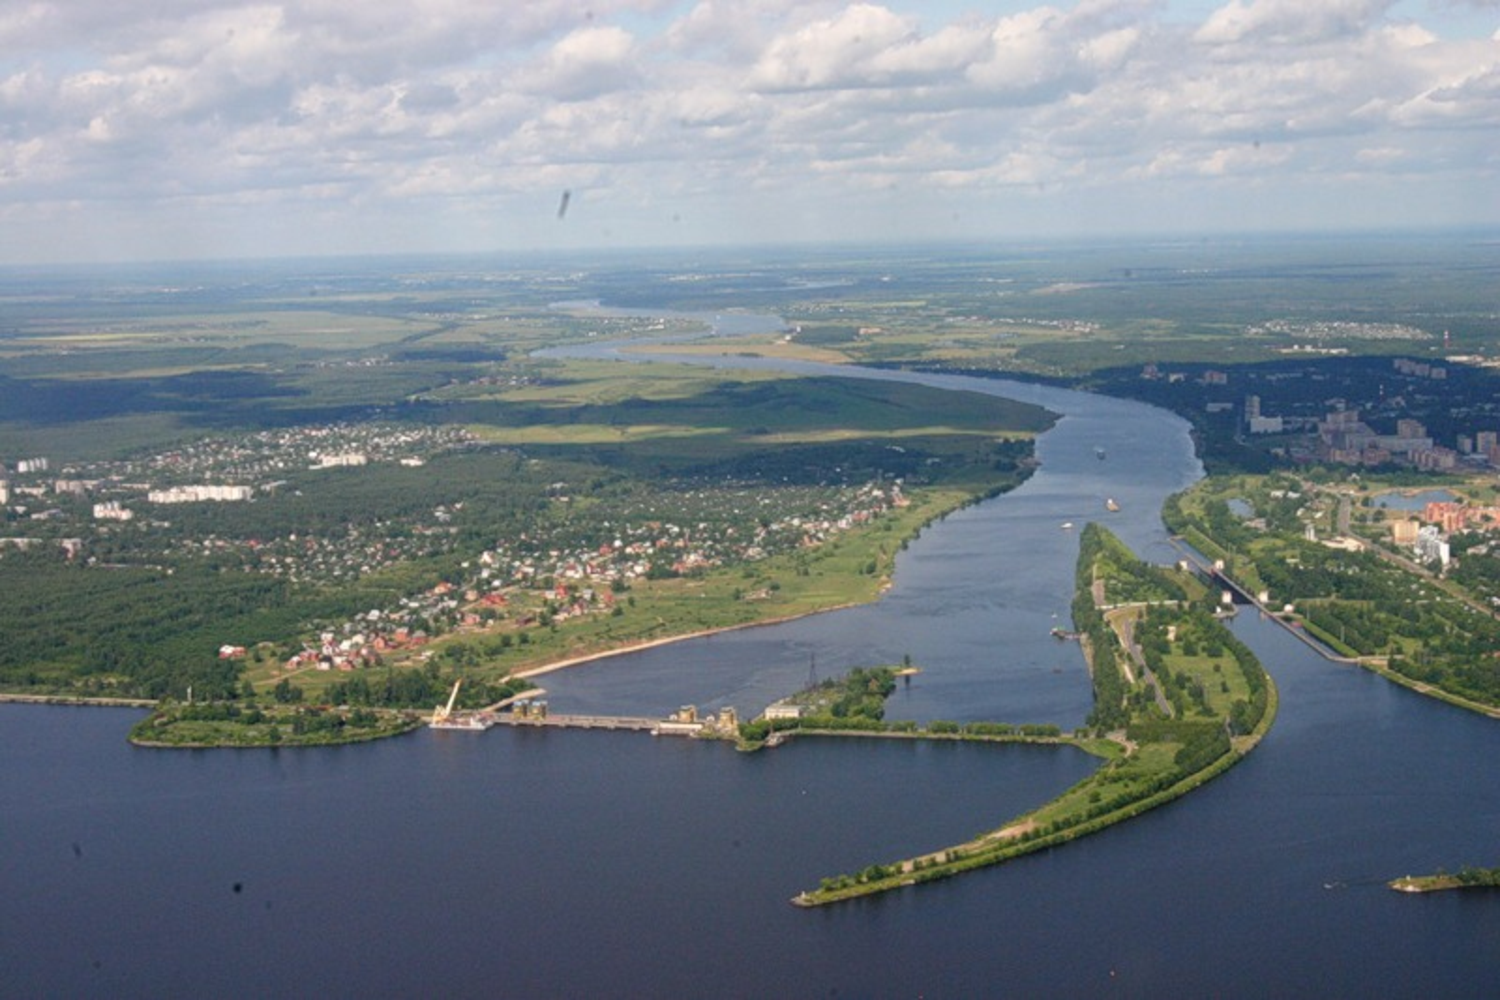
\includegraphics[scale=0.25]{dubna_town.pdf}}{}
%\addtobeamertemplate{title page}{\centering 
\includegraphics[scale=.05]{vblhep_logo.png}}{} 
%\addtobeamertemplate{title page}{\centering 
\includegraphics[scale=0.095]{wpcf2018_2.png}}{}
\vskip -1cm
\title[\bf Poland, Warsaw, III NICA DAYS 2019, MPD Collaboration meeting]
      {\textbf{\large {{\color{darkred!70!black} Correlation femtoscopy and factorial moments at the NICA energies}}}}
      \author[\bf P.~Batyuk]{\textit{\textbf{{\footnotesize \underline{P.~Batyuk$^{1}$}, M. Cheremnova$^{2}$, O. Kodolova$^{2}$, L. Malinina$^{1, 2}$,
              K. Mikhaylov$^{1, 3}$, G.Nigmatkulov$^{4}$, G. Romanenko$^{2}$}}}} 
      %on behalf of the MPD collaboration} 
      \institute{\bf on behalf of PWG3 (Correlations and Fluctuations) \\
        Supported by the RFBR grant 18-02-40044}
      \date{\tiny \bf $^{1}$Joint Institute for Nuclear Research, Dubna, Russia\\
        $^{2}$ Skobeltsyn Research Institute of Nuclear Physics, Moscow State University, Moscow, Russia\\
        $^{3}$ NRC Kurchatov Institute – ITEP, Rusian Federation, Moscow, Russia \\
        $^{4}$ National Research Nuclear University, Moscow Engineering Physics Institute, Moscow, Russia}  
      % \newpage \footnotesize April 14, 2016}}
   
      \graphicspath{{../common_figures/}}
      
      \begin{document}
      
      \maketitle
      \note{First of all, many thanks to organizers for a given opportunity to present a report withing the meeting. On behalf of the physics working group,
      mainly, from the part that is responsible for correlation studies, I would like to present our current status on studies of correlation femtoscopy at the NICA energies. Main contributors are presented in the slide. The work has been supported by the RFBR grant for a period of three years. Also, we decided to expand list of your studies, and first results on factorial moments extracted directly from the model we are using are presented in the report. }
      \begin{frame}
        \bf
        \frametitle{\bf \centering Outline:}
        \begin{itemize}
        \item Femtoscopy and Motivation
        \item Hybrid vHLLE+UrQMD model
        \item Comparison with STAR BES
        \item First look at factorial moments with vHLLE+UrQMD
        \item Probing some tests with the reconstructed MPD tracks  
        \item Other activities we are responsible for
        \end{itemize}
      \end{frame}

      \begin{frame}[shrink=40]
        \bf
        \vskip -.4cm
        \frametitle{\bf \centering Femtoscopy formalism}
        \begin{columns}[c]
          \column{.30\textwidth}
          \begin{block}{}
            \begin{figure}[H]
              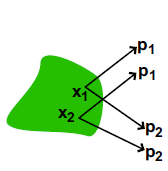
\includegraphics[width=1.\linewidth]{corr_femto1.png}
            \end{figure}
          \end{block}
          \column{.65\textwidth}
          \begin{block}{{\bf \centering Correlation femtoscopy:}}
            %     {\tiny
            Measurement of space-time characteristics $R$, $c_{\tau}$ of particle production
            using particle correlations due to the effects of quantum statistics (QS) and final state interactions (FSI)
            %      }
          \end{block}
          \begin{block}{{\bf \centering Two-particle correlation function:}}
            %      \tiny{
            \begin{center}
              {\bf theory:     $C(q) = \dfrac{N_{2}(p_{1}, p_{2})}{N_{1}(p_{1}) N_{2}(p_{2})}, C(\infty) = 1$
                
                experiment: $C(q) = \dfrac{S(q)}{B(q)}, q = p_{1} - p_{2}$
                
                \alert {S(q)} is a distribution of pair momentum difference of particles from the same event
                
                \alert {B(q)} is a reference distribution built by mixing of particles from different events}
            \end{center}
            %     }
          \end{block}
        \end{columns}
        \vskip -0.1cm
        \begin{columns}[t]
          \column{.45\textwidth}
          \begin{block}{\bf \centering Parametrizations used:}
            %\footnotesize
            % \begin{block}{\bf \centering 1D CF:}
            \centering 1D CF: \\
            \centering $C(q_{inv}) = 1 + \lambda e^{-R^{2} q_{inv}^{2}}$ \\
            $R$ is a Gaussian radius in PRF, \\
            $\lambda$ is a correlation strength parameter

            {\alert{1D-analysis}} is sensitive only to the system size averaged over all directions.\\
            \centering 3D CF: \\
            % \end{block}
            %  \begin{block}{\bf \centering 3D CF:}     
            \centering $C(q_{out}, q_{side}, q_{long}) = 1 + \lambda e^{-R_{out}^{2}q_{out}^{2} - R_{side}^{2}q_{side}^{2} - R_{long}^{2}q_{long}^{2}}$ \\
            Both R and \bf{q}  are in Longitudinally Co-Moving Frame (LCMS) \\
                        
            {\alert{3D-analysis}} gives an access to the three system sizes in three directions separately.
            %  \end{block}
          \end{block}
          \column{.49\textwidth}
          \begin{block}{\center \bf Definition of femtoscopy radii:}
            \begin{figure}[H]
              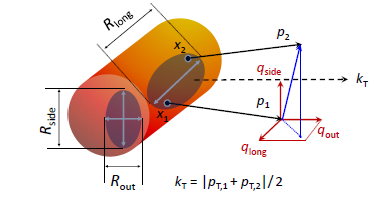
\includegraphics[width=.9\linewidth]{corr_femto4.png}
            \end{figure}
            \vskip -0.5cm
            S. Pratt. Phys. Rev. D 33 (1986) 1314 \\
            G. Bertsch. Phys. Rev. C37 (1988) 1896
          \end{block}
        \end{columns}
        \note{
          Correlation femtoscopy allows one to perform measurements of space-time characteristics of particle production taking into account the effects
          of quantum statistics and final state interactions. In the report I will speak on two-particle correlation femtoscopy only.  A standard formalism on
          experimental definition of two-particle correlation function is presented in the slide. In the results I am presenting, a 3D-parameterization of
          correlation function has been used, so, we have access to three system sizes in three directions separately.}
      \end{frame}

\begin{frame}
        \bf 
        \vskip -0.5cm
        \frametitle{\bf \centering Motivation}
                   {\footnotesize 
                     \begin{columns}[t]
                       \column{.49\textwidth}
                       \begin{block}{}
                         \begin{itemize}
                         \item {\color{darkred!70!black} Femtoscopy allows one:}
                           \begin{itemize}
                           \item {\footnotesize To obtain spatial and temporal information on particle-emitting source at kinetic freeze-out}
                           \item {\footnotesize To study collision dynamics depending on EoS}
                           \end{itemize}
                         \end{itemize}
                         
                         \begin{itemize}
                         \item {\color{darkblue!70!black} RHIC Beam Energy Scan program (BES-I):} $\sqrt{s_{NN}}$ = 7.7, 11.5, 19.6, 27, 39 GeV \\
                           Measured pion and kaon femtoscopic parameters: $m_{T}$-dependences of radii, flow-induced $x-p$ correlations
                         \item {\color{darkgreen!50!black} NICA energy range:} $\sqrt{s_{NN}}$ = 4 - 11 GeV
                         \end{itemize}
                       \end{block}
                       \column{.3\textwidth}
                       \begin{block}{\bf \centering {\tiny Phys. Rev. C92 (2015) 1, 014904}}
                         \begin{figure}[H]
                           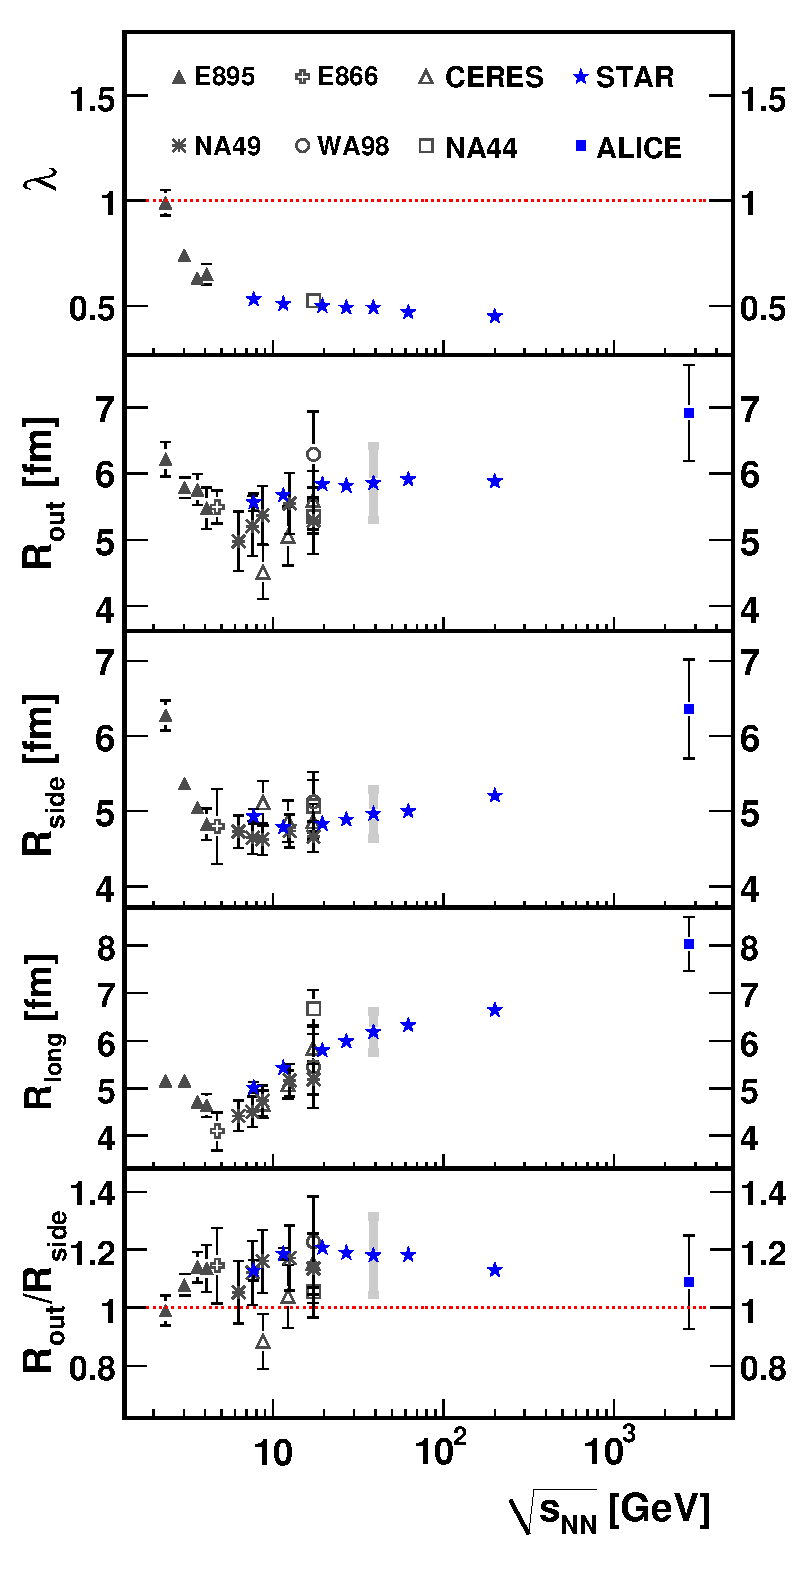
\includegraphics[width=1.\linewidth]{RiRootS.eps}
                         \end{figure}
                       \end{block}
                     \end{columns}
                   }
                   \note{In the slide the extracted femtoscopic radii are presented as a function of collision energy in c.m.s. for different experiments.
                     Within the BES program at RHIC for a wide set of collision energies were measured different femtoscopic observables, like $m_{T}$-dependence of
                     radii, for kaons and pions. In the NICA energy range the observed behaviour of some observables, like ratio of $R_{out} / R_{side}$,
                   which is sensible to emission duration, does not look monotonic.
                   Taking into account a fact on possible scenarios concerning a nuclear matter EoS to be realized in this energy region and some theoretical
                   considerations on existence of the Critical Point, an extended study of femtoscopic observables in the NICA energy range looks very promising,
                   since it can give us more understanding of collision dynamics depending on EoS.}   
\end{frame}

\begin{frame}
        \bf
        \frametitle{\bf \centering Femtoscopy with vHLLE+UrQMD}
        \vskip -.3cm
        \begin{block}{\bf \centering Iu. Karpenko, P. Huovinen, H.Petersen, M. Bleicher, Phys.Rev. C 91, 064901 (2015)}
          \begin{figure}[H]
            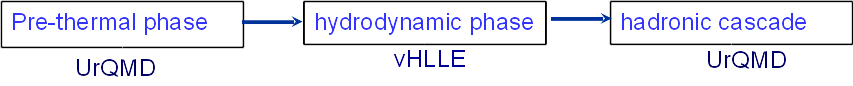
\includegraphics[width=1.\linewidth]{vHLLE_UrQMD_sandwich.png}
          \end{figure}
        \end{block}
        \vskip -.8cm
        \begin{columns}[t]    
          \column{.30\textwidth}
          \begin{block}{\bf \centering {\tiny Parameters $\tau_0$, $R_\perp$, $R_\eta$ and $\eta/s$ adjusted using basic
                observables in the RHIC BES-I region.}}        
            %\vskip -.3cm
            \resizebox{\columnwidth}{!}{%       
              \begin{tabular}{|l|l|l|l|l|}
                \hline
                $\sqrt{s_{\rm NN}}$~[GeV] & $\tau_0$~[fm/c] & $R_\perp$~[fm] & $R_\eta$~[fm] & $\eta/s$ \\ \hline
                7.7          &      3.2        &     1.4        &     0.5    &    0.2   \\ \hline
                8.8 (SPS)    &      2.83       &     1.4        &     0.5    &    0.2   \\ \hline
                11.5         &      2.1        &     1.4        &     0.5    &    0.2   \\ \hline
                17.3 (SPS)   &      1.42       &     1.4        &     0.5    &    0.15  \\ \hline
                19.6         &      1.22       &     1.4        &     0.5    &    0.15  \\ \hline
                27           &      1.0        &     1.2        &     0.5    &    0.12  \\ \hline
                39           &      0.9        &     1.0        &     0.7    &    0.08  \\ \hline
                62.4         &      0.7        &     1.0        &     0.7    &    0.08  \\ \hline
                200          &      0.4        &     1.0        &     1.0    &    0.08  \\ \hline
              \end{tabular}
            }
            \vskip 0.2cm
                   {\color{darkred!70!black} \scriptsize Model tuned by matching with existing experimental data from SPS and BES-I RHIC}
          \end{block}

          \column{.32\textwidth}
          \begin{block}{\bf \centering \scriptsize EoS to be used in the model}
            \begin{itemize}
            \item \tiny Chiral EoS - crossover transition \\ J. Steinheimer et al., J. Phys. G 38, 035001 (2011)
            \item \tiny Hadron Gas + Bag Model 1-st order phase transition \\ P. F. Kolb et al., Phys.Rev. C 62, 054909 (2000)
            \end{itemize}
          %  \vskip -.15cm
          %  \begin{figure}[H]
          %    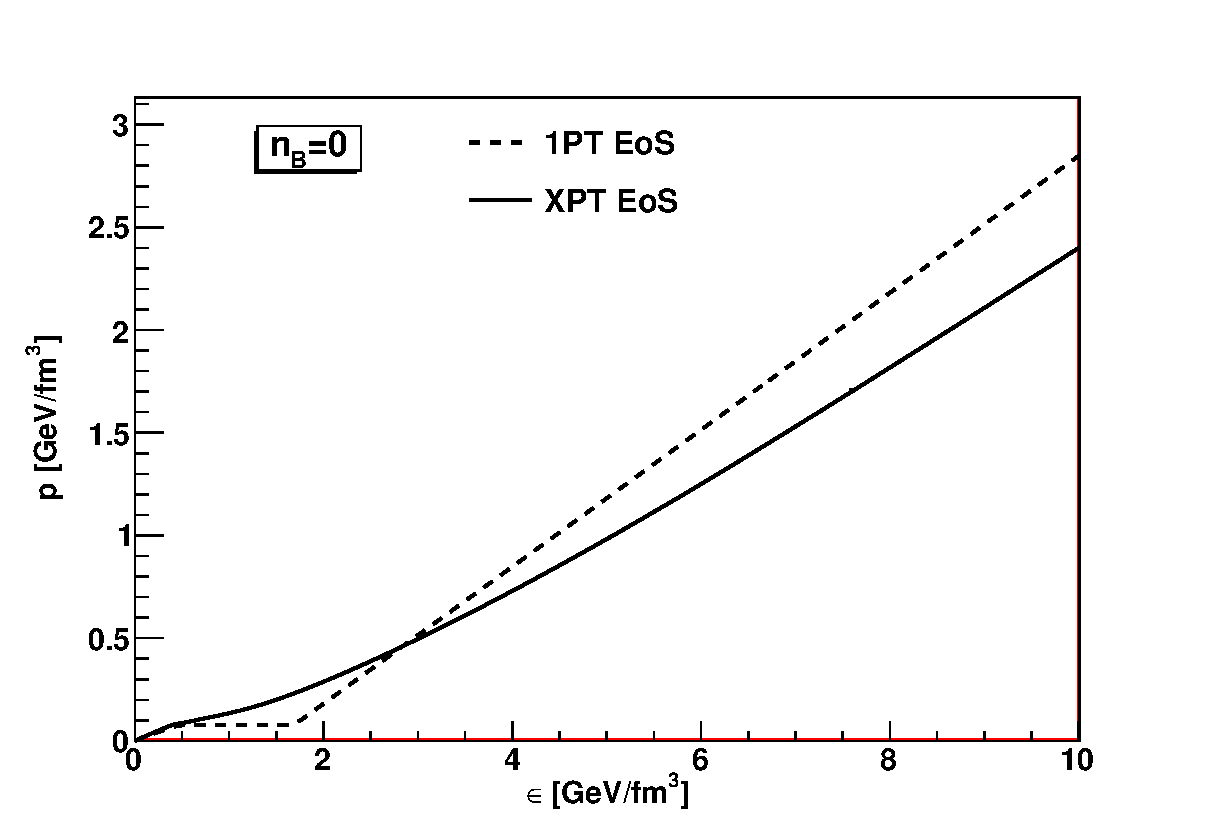
\includegraphics[width=1.01\linewidth]{eos.eps}
          %  \end{figure}
          \end{block}
          \vskip -0.4cm
          \begin{block}{}
            {\scriptsize {\color{darkblue!70!black} Hydrodynamic phase lasts longer with 1PT,
                especially at lower energies but cascade smears this difference.}}
          \end{block}

          \column{.32\textwidth}  
          \begin{block}{\bf \centering {\tiny Pion emission time}}
            \vskip -0.1cm
                   {\tiny
                     (a) - after hydrodynamic phase \\
                     (b) - after cascade
                   }
                  % \vskip -0.45cm
                   \begin{figure}[H]
                     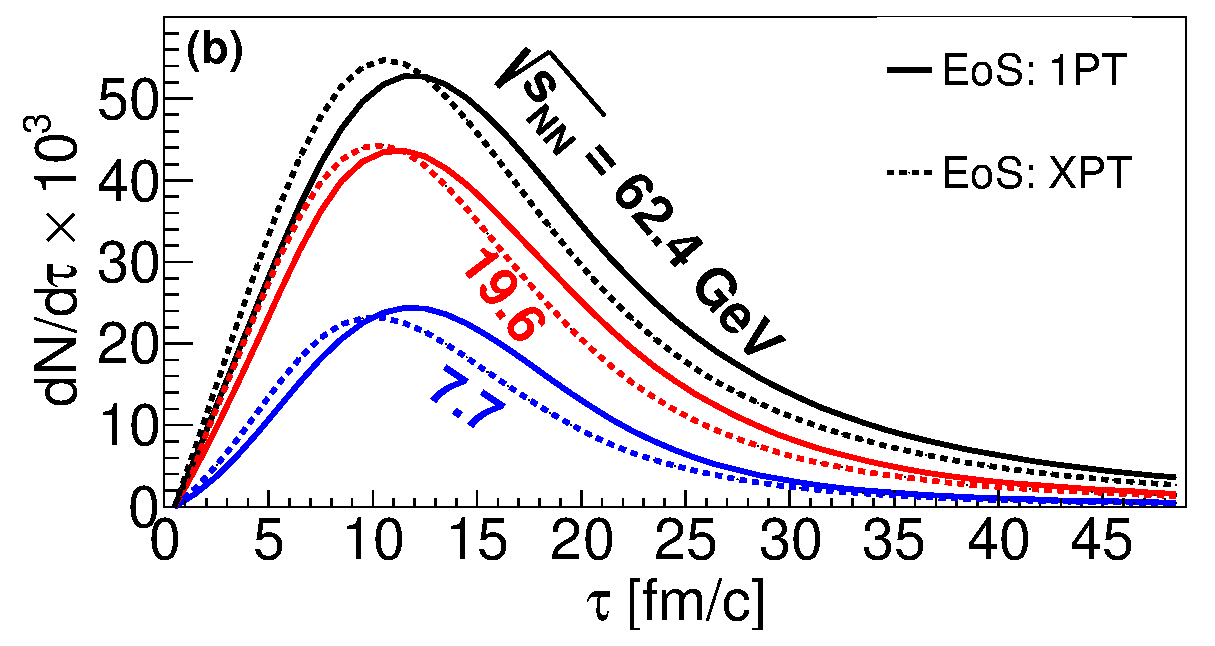
\includegraphics[width=1.\linewidth]{fig1a.eps} \\
                     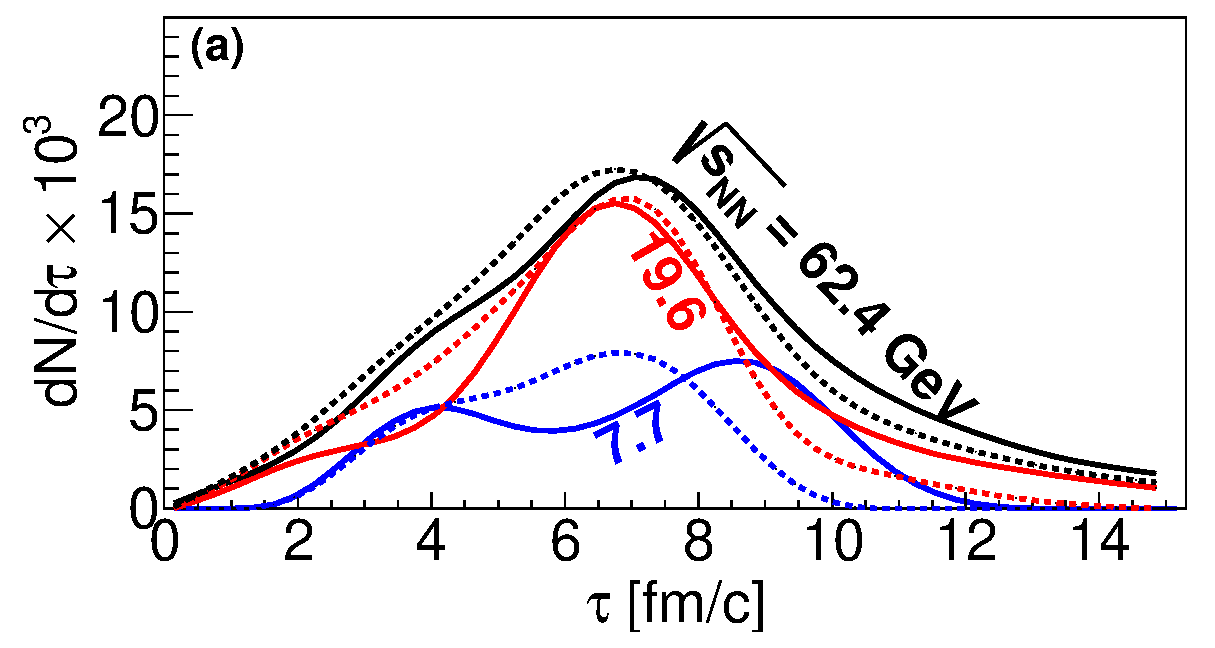
\includegraphics[width=1.\linewidth]{fig1b.eps}
                   \end{figure}
                   %\vskip -.7cm
          \end{block}
        \end{columns}
        \vskip -.3cm
        \begin{columns}[t]
          \column{.42\textwidth}
          %\begin{block}{\bf \centering {\tiny Ratios of 1D-projections of 3D correlation functions for two EoS}}
          %  \vskip -.2cm
          %  \begin{figure}[H]
          %    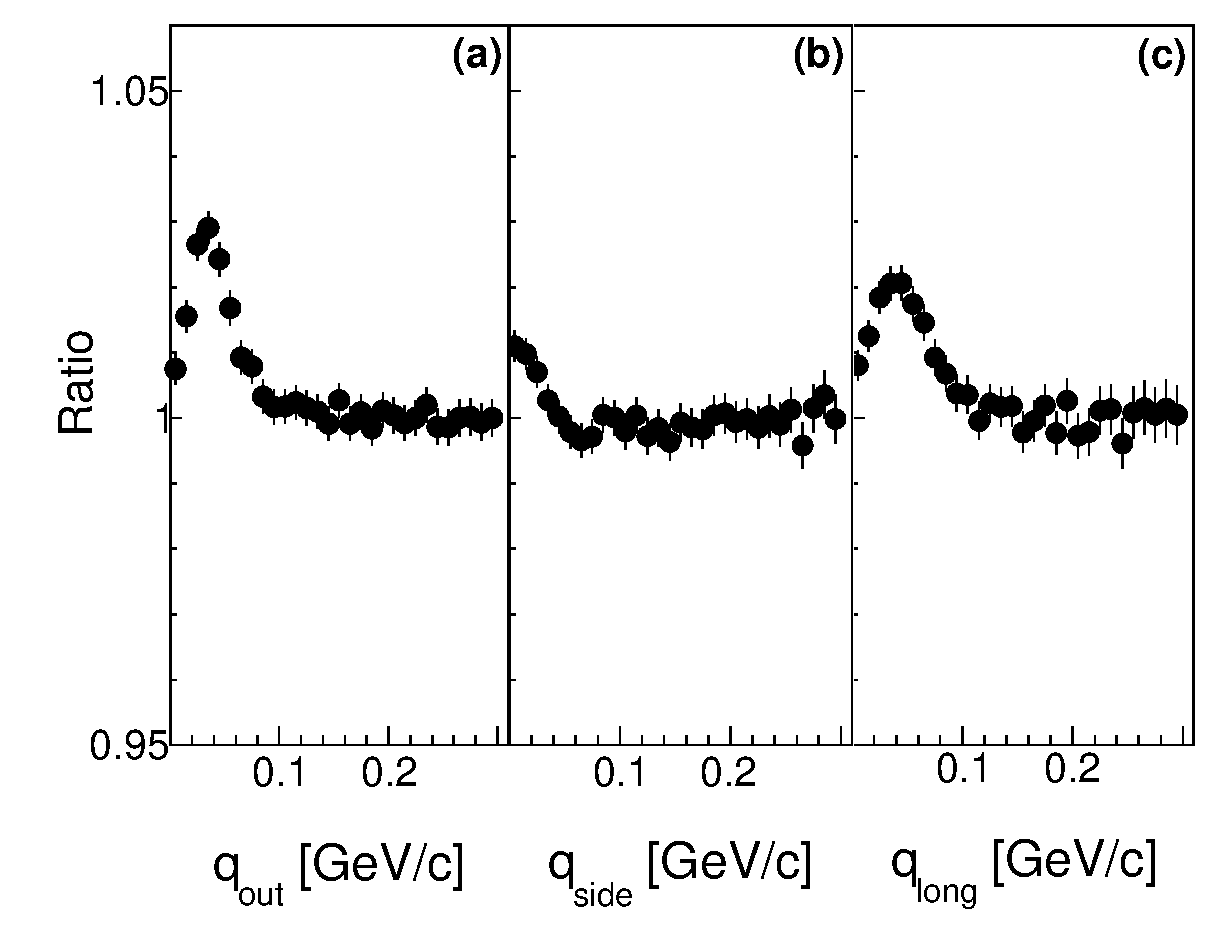
\includegraphics[width=1.0\linewidth]{fig3.eps}
          %  \end{figure}
          %\end{block}
          \column{.49\textwidth}
          %       {\footnotesize
          %         \begin{block}{\bf \centering Analysis:}
          %           \begin{center}
          %            AuAu @ $\sqrt{s_{NN}} = 7.7$ GeV \\
          %            Centrality 0-5\% \\
          %            $k_{T} = (0.15-0.25)$ GeV/c
          %          \end{center}
          %        \end{block}
          %        \vskip -.3cm
          %        \begin{block}{}
          %          \begin{itemize}
          %          \item Difference is seen in the ``out'' and ``long''
          %            directions.
          %          \item Ratios in the ``out'' and ``long'' directions reach values up to 1.03 at small
          %            $q_{out}$ and $q_{long}$.
          %          \end{itemize}
          %        \end{block}
          %      }
        \end{columns}
        \note{
          \vskip -0.6cm
          \scriptsize As a candidate for our studies the vHLLE+UrQMD model has been chosen. It is a model of ``sandwich''-like type
          consisting of three stages to be used sequentially for describing collision evolution. Initial stage of collision and hadronic cascade are realized via UrQMD model,
          meanwhile hydrodynamic stage includes calculations done by the author of the model. To get more detail on it, one is reffered to the publication. The model allows one to
          perform calculations assuming two different scenarios of nuclear matter EoS to be used, croosover and a first order phase transition. Basic parameters of the model
          have been tuned using experimental data from SPS and the BES program. The tuning aimed to describe reasonably well basic particle spectra, but did not cover femtoscopic
          observables. So, femtoscopy observables derived from the model are free ones and not restricted by any "femtoscopy" adjustments.
          The main reason that convinced us to use the model for our studies is a visible difference in emission of particles, depending on the EoS used, as after hydrodynamic phase
          well as hadronic cascade. The energy is lower the difference is bigger one can observed after the hydrodynamic stage. Despite the hadronic cascade smears the difference,
          it still remains visible, thus it could lead to different behaviour of femtoscopic observables depending on EoS.}
      \end{frame}
      

     

    \begin{frame}
        \bf
        \frametitle{\bf \centering 3D Pion radii versus $m_{T}$ with vHLLE+UrQMD }
        \begin{columns}[c]
          \column{.36\textwidth}
          \vskip -.3cm
          
          % \vskip -.75cm
          \begin{block}{{\bf \scriptsize  Phys. Rev. C 96, 024911 (2017)}}
            \begin{figure}[H]
              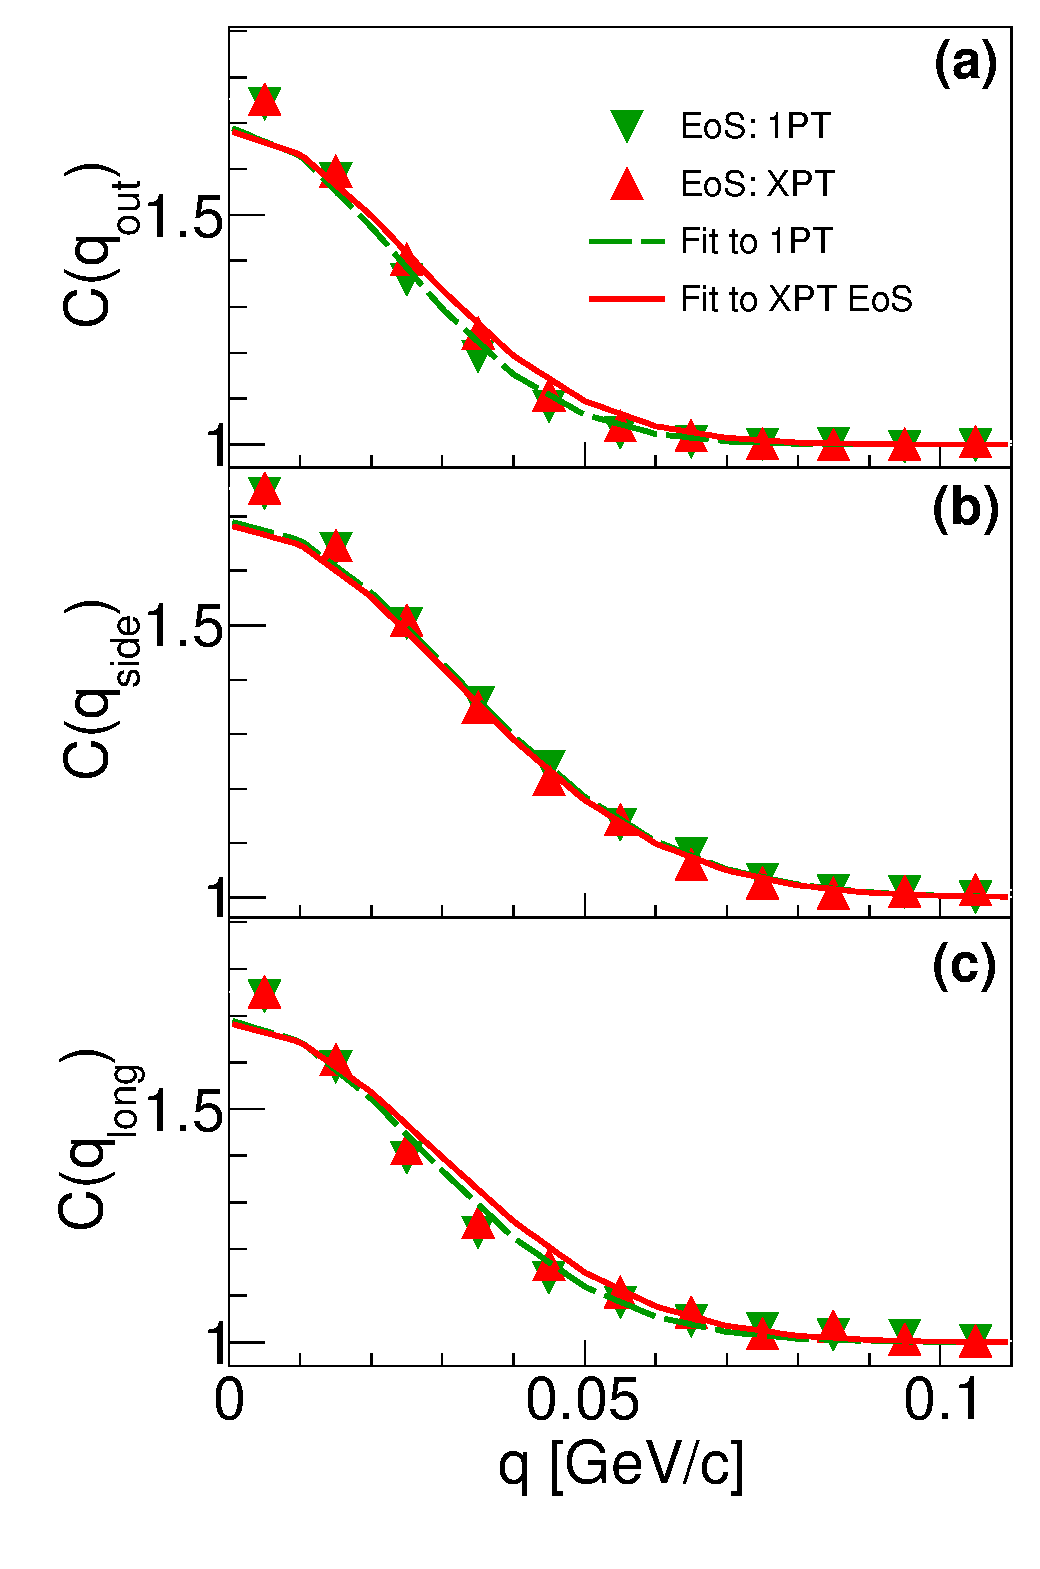
\includegraphics[width=1.\linewidth]{fig2.eps}
            \end{figure}
          \end{block}
          \column{.63\textwidth}
          \vskip -.3cm
          \begin{block}{\bf \centering {\tiny Comparison of extracted radii with the STAR data}}
            % \vskip .3cm
            \begin{figure}[H]
              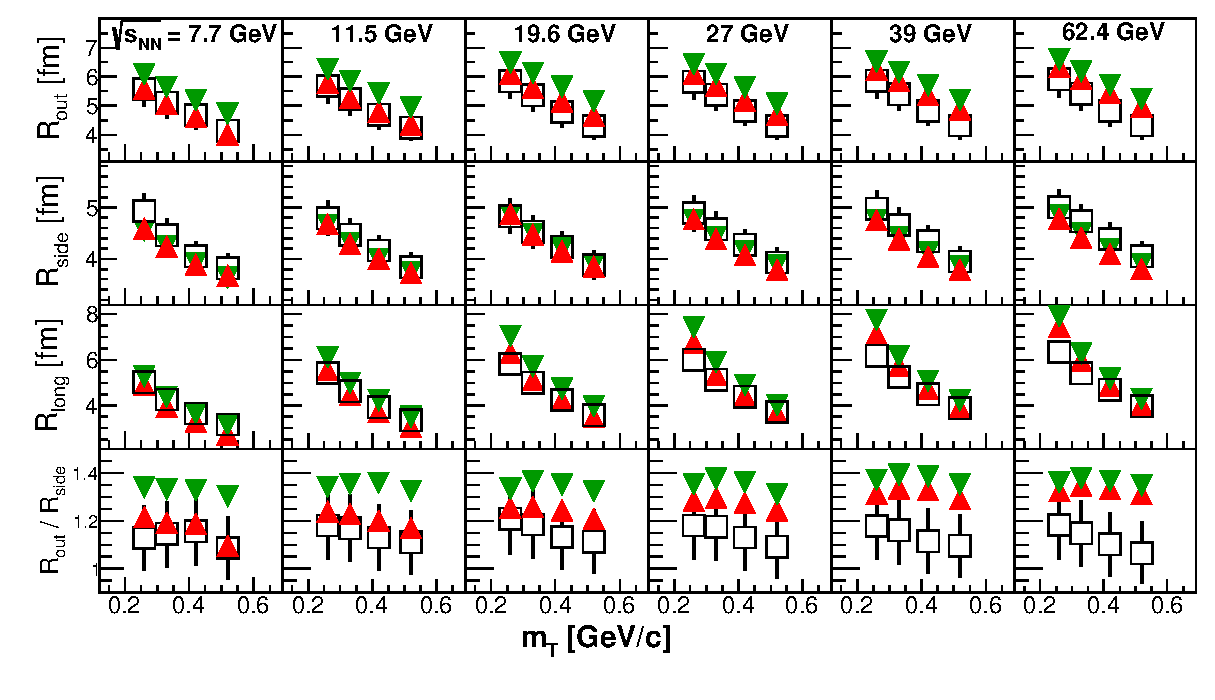
\includegraphics[width=1.0\linewidth]{fig4_poster.eps}
            \end{figure}
          \end{block}
          % \begin{block}{}
          %   {\scriptsize
          %     \begin{itemize}
          %     \item {\color{darkred!70!black} EoS with a crossover in the fluid phase} results in a quite reasonable reproduction of 3D pion femtoscopic radii measured by
          %       the STAR collaboration (empty squares).
          %     \item {\color{darkgreen!50!black} EoS with a first-order phase transition} leads to fact that the ``out'' and ``long'' Gaussian femtoscopic radii are systematically larger
          %      if comparing with the {\color{darkred!70!black} crossover EoS}; the ``side'' radii coincide for both types of EoS.
          %  \end{itemize}
          % }
          %\end{block}
          \vskip -.35cm
          \begin{block}{}
            {\color{darkred!70!black} Crossover EoS} ``works'' better for lowest collision energies.
          \end{block}
          \vskip -.35cm
          \begin{block}{}
            {\scriptsize
              \begin{itemize}
              \item $R_{out}$ (XPT) at high energies and $R_{out}$ (1PT) at all energies are slightly overestimated
                %$\rightarrow$
                %{\color{darkred!70!black} an indication to reduce the emission time in the model.}
              \item $R_{out, long}$ (1PT) > $R_{out, long}$ (XPT) by value of $\sim$ 1-2~fm. 
              \end{itemize}
            }
          \end{block}
        \end{columns}
        \note{
          Since we chose a model to be used for our studies, the first step
          we did, was to extract femtoscopic radii directly from the model
          to compare them with existing eperimental data. As a data base,
          we took the pion STAR data got from the RHIC BES program.
          Calculations with the crossover EoS are presented by red color,
          meanwhile those for the 1PT scenario - by green color. If
          comparing between both scenarios, one can see that the crossover
          scenario work better for the radii description, especially,
          when considering $R_{out} / R_{side}$ ratio at lowest energies
          available. 1PT-scenario overestimates the radii by value of about
          1fm for out and long direction. THhis fact could be considered as
          an indication to reduce the emission time in the model.
        }
      \end{frame}

      \begin{frame}
        \frametitle{\bf \centering $R_{out} / R_{side}$  with vHLLE + UrQMD model}
        \bf
        \vskip -1.3cm
        \begin{columns}[t]
          \column{.35\textwidth}
          \begin{block}{}     
            \begin{figure}[H]
              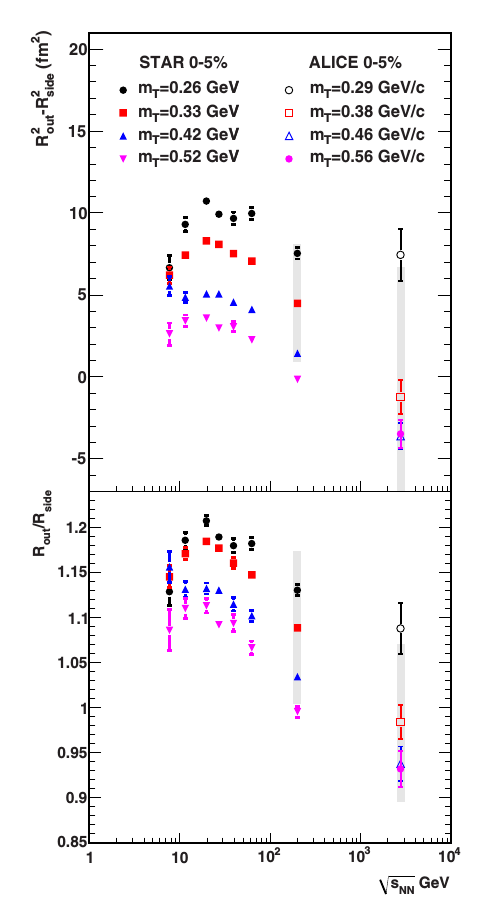
\includegraphics[width=1.0\linewidth]{RoutRside_STAR_ALICE.png}
            \end{figure}
          \end{block}

         % \column{.3\textwidth}
         
         % \vskip -0.25cm
          %\begin{block}{\bf \centering Model calculations:}
          %  \begin{itemize}
          %  \item \scriptsize Optimal description of the femtoscopic radii
          %  requires about 1~fm shorter duration of pion emission with the present setup of the model.       
          %  \end{itemize}
          %\end{block}
          
          \column{.48\textwidth}
                 {\scriptsize 
                   \begin{block}{\bf \centering \scriptsize Exp. data:}
                     $R_{out} / R_{side}$ and $R_{out}^{2} - R_{side}^{2}$ as a function of
                     $\sqrt{s_{NN}}$ at a fixed $m_{T}$ demonstrate a wide maximum near
                     $\sqrt{s_{NN}} \approx$ 20 GeV
                   \end{block}
                 }
                 \vskip -0.4cm
                 \begin{block}{\bf \centering \scriptsize Our calculations (performed at $m_{T}$ = 0.26 GeV, 0-5\%): }
                   \vskip -.25cm
             \begin{figure}[H]
               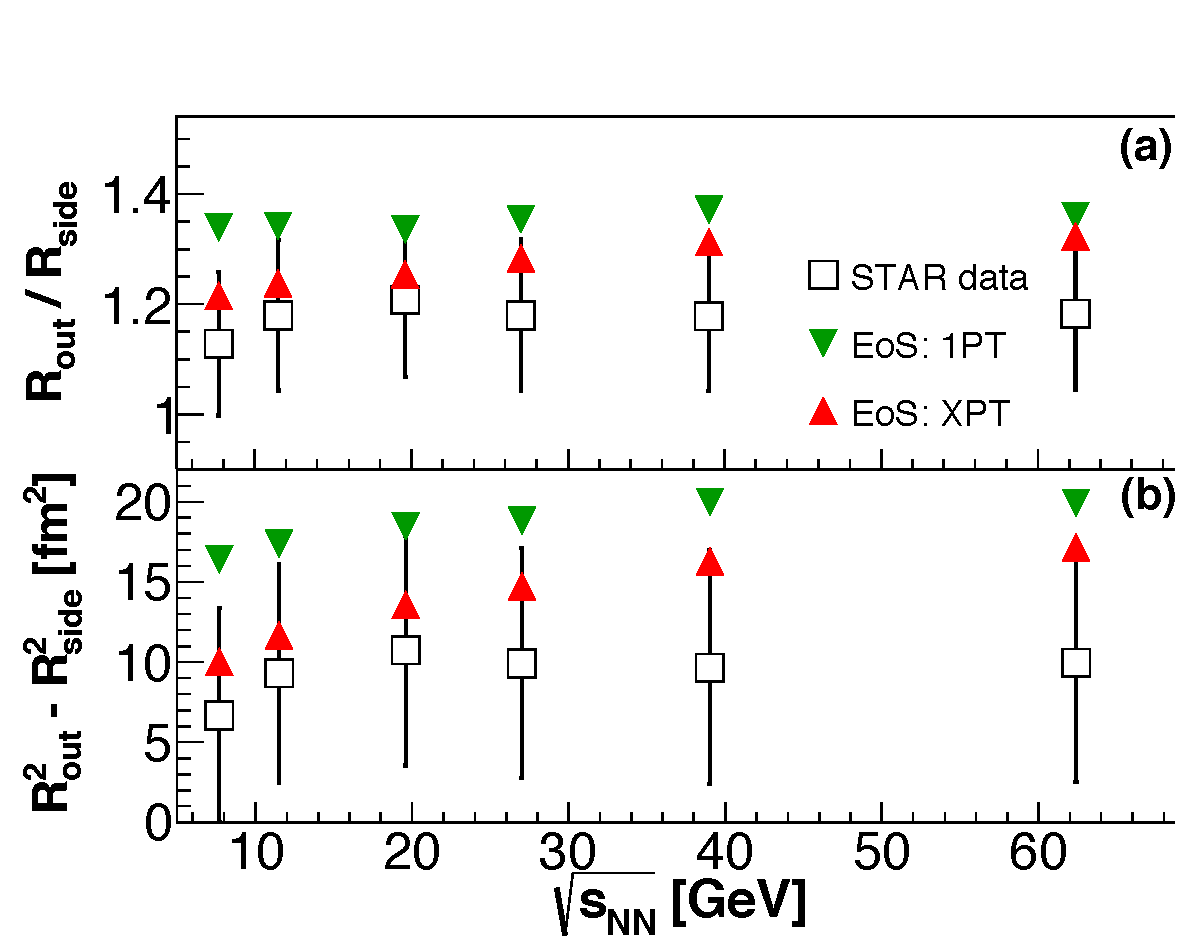
\includegraphics[width=1.0\linewidth]{fig5_modif.pdf}
             \end{figure}
             \vskip -0.65cm
             {\scriptsize $R_{out} / R_{side}$ (XPT) agrees with almost all STAR data points within rather large systematic errors,
             while $R_{out} / R_{side}$ (1PT) overestimates the data.}
          \end{block}
        \end{columns}
        \vskip -1.cm
       % \begin{columns}[t]
        %  \column{.33\textwidth}
        %  \column{.64\textwidth}
         % \begin{block}{}
           % \begin{itemize}
         % \item
          %  {\color{darkred!70!black} Does a new set of parameters help us to accommodate the femtoscopic radii?}
          %  \end{itemize}
       %   \end{block}
       % \end{columns}
        \note{Another point we got from the model covers not only
          $R_{out} / R_{side}$ but difference of its squares. This part of
        analysis was motivated by the fact that the difference at a fixed
        $m_{T}$-value shows a wide maximum around 20 GeV of collision energy in
        c.m.s. as obtained from experimental data. Calculations we performed are
        agreed with the STAR data points with large systematic errors if assuming
        the crossover scenario in the model. 1PT-scenario overestimates as ratio
        as well as difference of considering radii.
        }
      \end{frame}

      
      \begin{frame}
        \bf
        \frametitle{Ratio of $R_{out, side, long}(1PT) / R_{out, side, long}(XPT)$ vs. $\sqrt{s_{NN}}$}
        \vskip -0.75cm
        \begin{columns}[t]
          \column{.38\textwidth}
          \begin{block}{}
             \begin{figure}[H]
               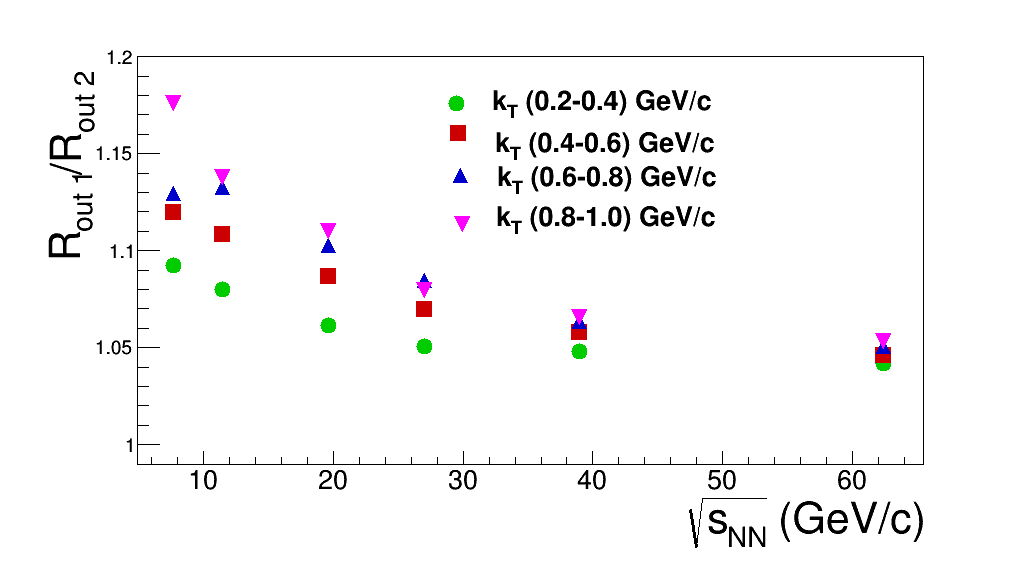
\includegraphics[width=1.0\linewidth]{Rout_diffEoS.png} \\
            % \end{figure}
            %  \begin{figure}[H]
               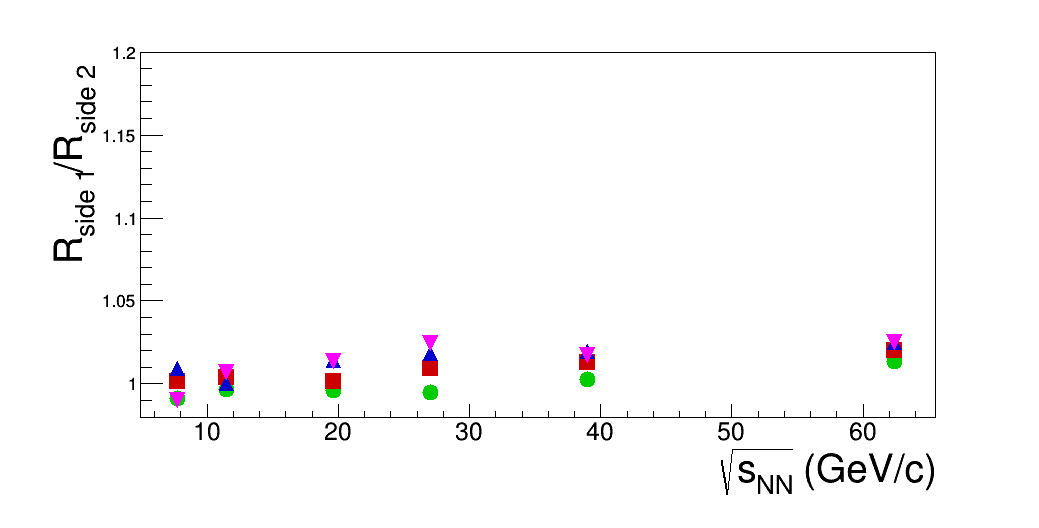
\includegraphics[width=1.0\linewidth]{Rside_diffEoS.png} \\
             % \end{figure}
             %  \begin{figure}[H]
               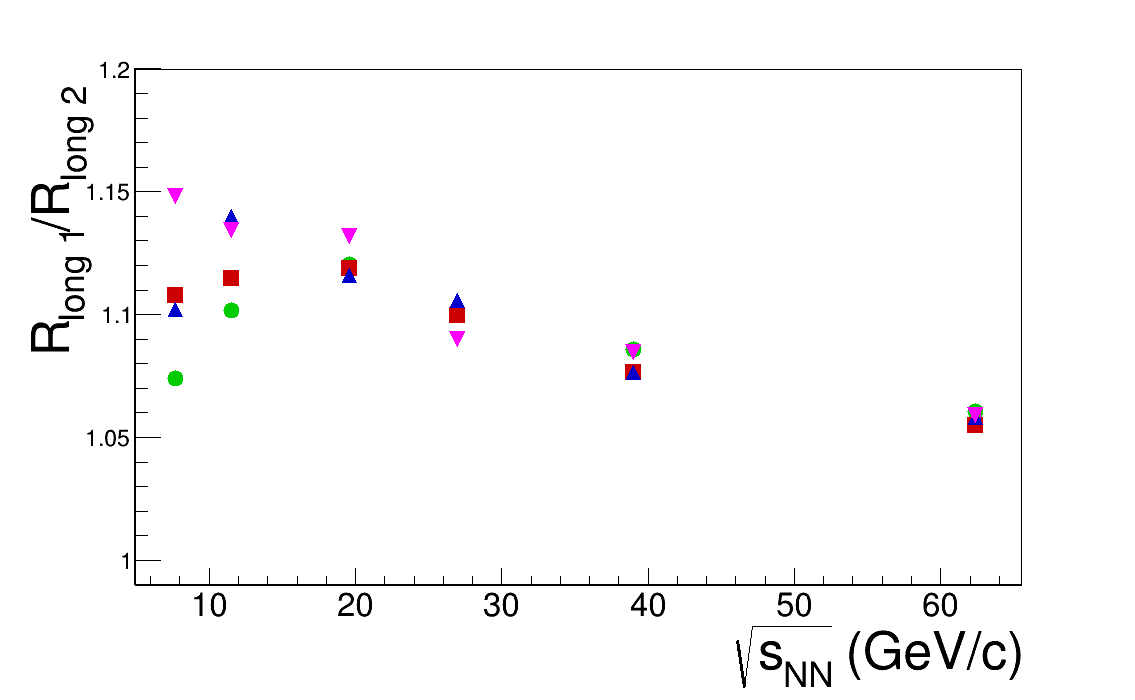
\includegraphics[width=1.0\linewidth]{Rlong_diffEoS.png}
             \end{figure}
          \end{block}
          \column{.49\textwidth}
          \begin{block}{}
            \begin{itemize}
            \item $R_{side}$ practically coincide for both scenarios
            \item $R_{out}$ and $R_{long}$  for 1PT EoS are greater than for XPT EoS 
              demonstrating a strong $k_{T}$-dependence
            \end{itemize}
          \end{block}
          \begin{block}{\bf \centering Why?}
            The difference comes from a {\color{darkred!70!black} weaker transverse flow developed in the fluid phase}
            with 1PT EoS as compared to XPT EoS  and its {\color{darkred!70!black} longer lifetime} in 1PT EoS
          \end{block}
        \end{columns}
        \note{
          In the slide ratios of corresponding radii for the 1PT and crossover
          scenarios are presented. Transverse momenta of pion pair are divided into
          four bins. $R_{side}$ has practically the same order of magnitude
          for both scenarios.
          $R_{out}$ and $R_{long}$ tend to be greater for the 1PT-scenario and
          demonstrate a clear $k_{T}$-dependence especially for lowest values of
          $k_{T}$. A weaker transverse flow in the fluid phase
          and its longer lifetime in the 1PT EoS if comparing with the crossover
          EoS could be considered as a possible explanation. 
        }
      \end{frame}
      
      \begin{frame}
        \bf
         \frametitle{\bf \centering \footnotesize Kaon correlation functions with vHLLE+UrQMD { \color{darkred!70!black} (NEW!)}}
         \vskip -.75cm
         \begin{columns}[t]
           \column{.50\textwidth}
           \begin{block}{\bf \centering Pions:}
             \begin{figure}[H]
               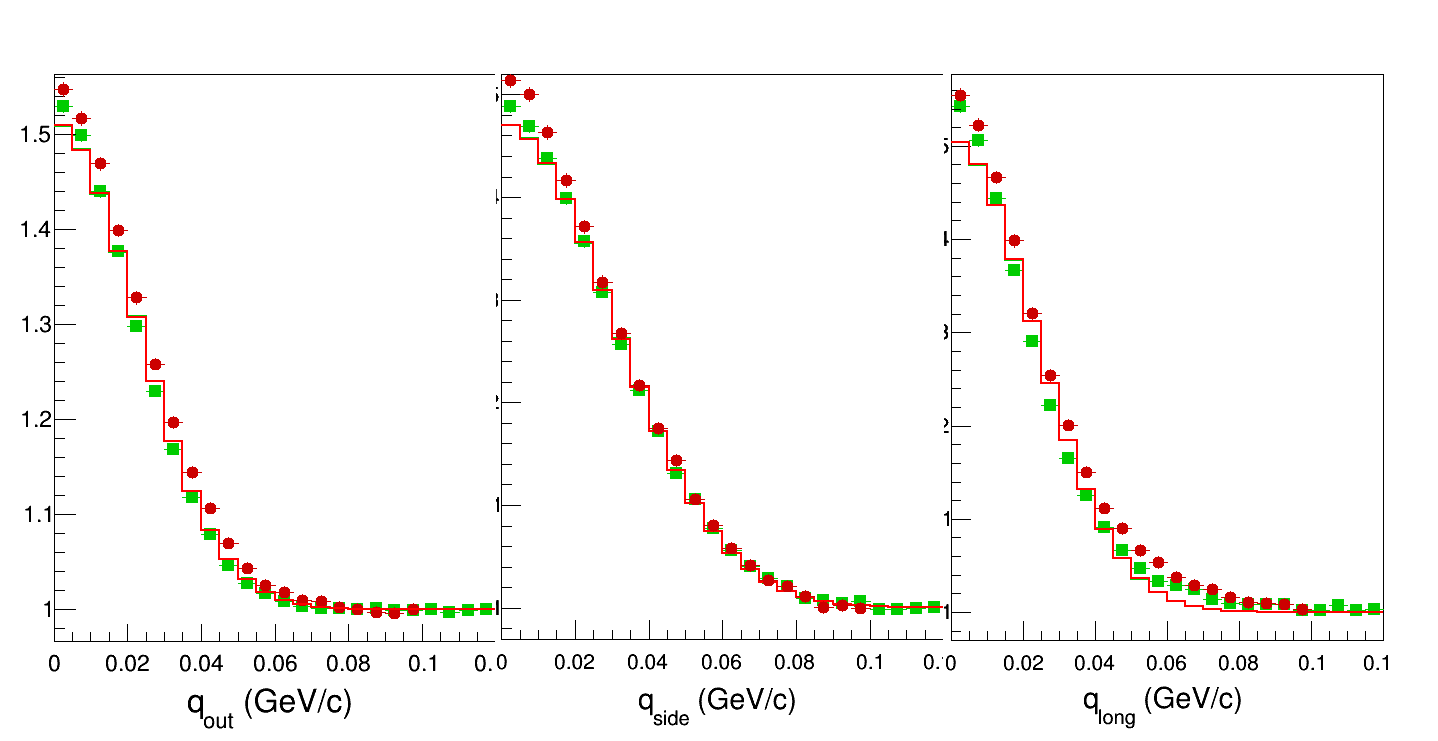
\includegraphics[width=1.0\linewidth]{proj3D_pions.png}
               \end{figure}
           \end{block}
            \vskip -.3cm
            \begin{block}{\bf \centering Kaons:}
             \begin{figure}[H]
                 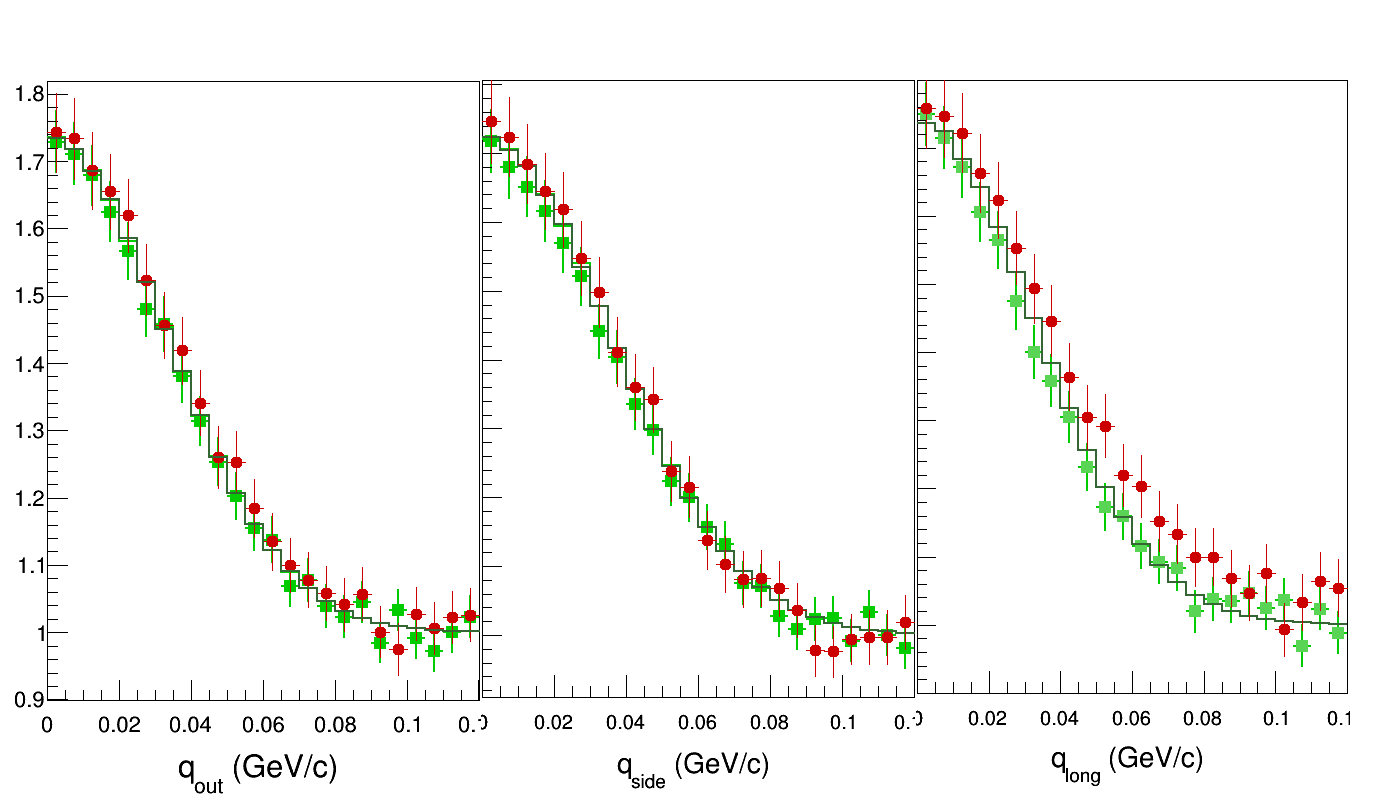
\includegraphics[width=1.0\linewidth]{proj3D_kaons.png}
             \end{figure}
           \end{block}
           \column{.39\textwidth}
           \begin{block}{\bf \centering Analysis:}
             \begin{itemize}
             \item \footnotesize AuAu, $\sqrt{s_{NN}} = 11.5$ GeV
             \item \footnotesize $N_{events} \approx 400 000$
             \item \footnotesize Standard 3D Gaussian fit used
             \end{itemize}
           \end{block}
           \vskip -.2cm
           \begin{block}{}
             \begin{itemize}
             \item Projections of {\color{darkred!70!black} 3D-kaon correlation functions} on out-side-long directions are {\color{darkred!70!black} more Gaussian}
             \item {\color{darkred!70!black} XPT CF projections} on {\color{darkred!70!black} long direction} are {\color{darkred!70!black} visibly wider} than 1PT especially {\color{darkred!70!black} for kaons}
             \end{itemize}
           \end{block}
         \end{columns}
         \note{
          As a continuation of our model studies and addition to the pion results,
          we have done a preliminary analysis for charged kaons. Details of the
          analysis are presented in the slide. The analysis revealed two remarkable
          facts. The first one states a more gaussian form of all projections
          of 3D correlation function for kaons. Also, in case of kaons long
          projection of correlation function is wider for the 1PT-scenario in the  model.
        }
      \end{frame}

      \begin{frame}
        \frametitle{\bf \centering Pion and kaon radii vs. $m_{T}$ with vHLLE+UrQMD}
        \vskip -.75cm
        \begin{columns}[t]
          \column{.55\textwidth}
          \begin{block}{}
          \begin{figure}[H]
            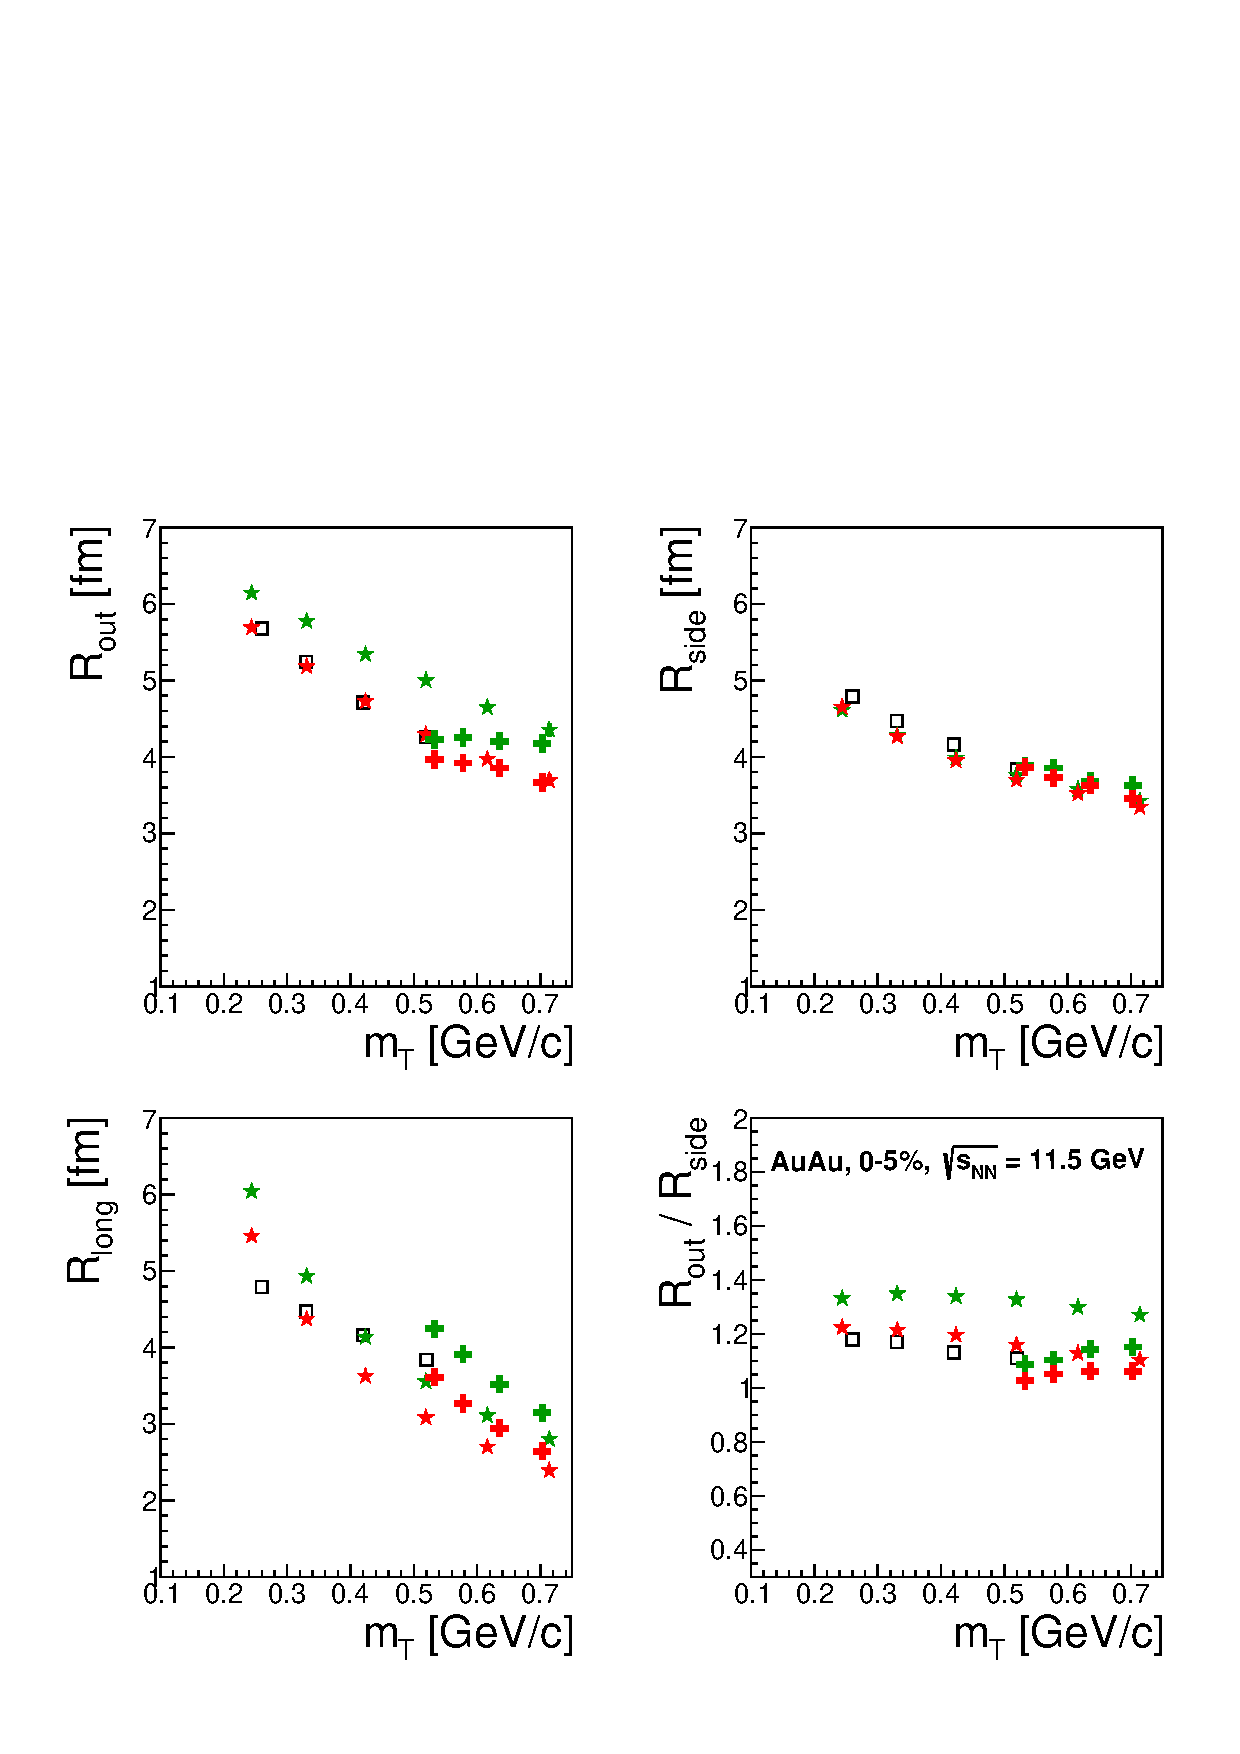
\includegraphics[width=1.\linewidth]{AuAu_115.pdf}
          \end{figure}
          \end{block}
          \vskip -.3cm
          \begin{block}{}
             \bf \color{darkred!70!black} Important to measure both kaon and pion radii!
          \end{block}
          \column{.315\textwidth}
          \begin{block}{}
            \bf
            \begin{itemize}
            \item \scriptsize As well as for pions kaon out and long radii are greater for 1PT than for XPT
            \item Approximate $m_{T}$-scaling for pions and kaons observed only for side radii
            \item Out almost flat for 1PT
            \item $R_{long}$(kaons) is greater than $R_{long}$(pions) due to larger average time emission
            \item $R_{out}$ / $R_{side}$ for kaons is less than for pions
            \item Approximately the same result is for AuAu $\sqrt{s_{NN}}$ = 7.7 GeV
            % \item Important to measure both kaon and pion radii
            \end{itemize}
          \end{block}         
        \end{columns}
      \end{frame}

        \begin{frame}
          \frametitle{\bf \centering Factorial moments with vHLLE+UrQMD}
          \vskip -.4cm
          \begin{block}{}
            \footnotesize
            \bf Proposed by A. Bialas and R. Peschanski (Nucl. Phys. B 273 (1986) 703) to study the dependence of the normalized factorial moments
            of the rapidity distribution on the size of the resolution
          \end{block}
          \vskip -.2cm
          \begin{columns}[t]
            \column{.05\textwidth}
            \column{.9\textwidth}
            \begin{block}{\bf \centering Set of definitions of moments and cumulants}
              \begin{equation*}
                F_{i} = M^{i-1} \cdot \left < \dfrac{\sum\limits_{j = 1}^{M} k_{j} \cdot (k_{j} - 1) \cdot ... \cdot (k_{j} - i + 1)}
                {N \cdot (N - 1) \cdot ... \cdot (N -i + 1)} \right >
              \end{equation*}          
            \end{block}
            \column{.05\textwidth}
          \end{columns}
          \vskip -.3cm
          \begin{columns}[c]      
          \column{.49\textwidth}
          \begin{block}{}
            \bf
             \footnotesize
          \begin{itemize}
          \item {\color {darkblue!70!black} No variation of moments $\delta y$ expected} if fluctuations are purely statistical
          \item {\color {darkred!70!black} Observation of variations indicates the presence of physics origin fluctuations}
          \end{itemize}
        \end{block}
          \column{.49\textwidth}
          \bf
          \begin{block}{}
            $M$ is the number of bins \\
            $\delta y$ is the size of mid-rapidity window
          \end{block}
          \vskip -.4cm
          \begin{block}{}
            \bf
             \footnotesize
            Intermittency ({\color{darkred!70!black} fluctuations of many different sizes in 1D, 2D and 3D space}) has been studied at LEP, Tevatron, Protvino in ee, hh, hA, AA
            interactions at various energies.
          \end{block}        
        \end{columns}
      \end{frame}

        \begin{frame}
          \frametitle{\bf \centering Factorial moments with vHLLE+UrQMD}
          \vskip -.75cm
          \begin{columns}[t]
            \column{.05\textwidth}
            \column{.7\textwidth}
            \begin{figure}[H]
              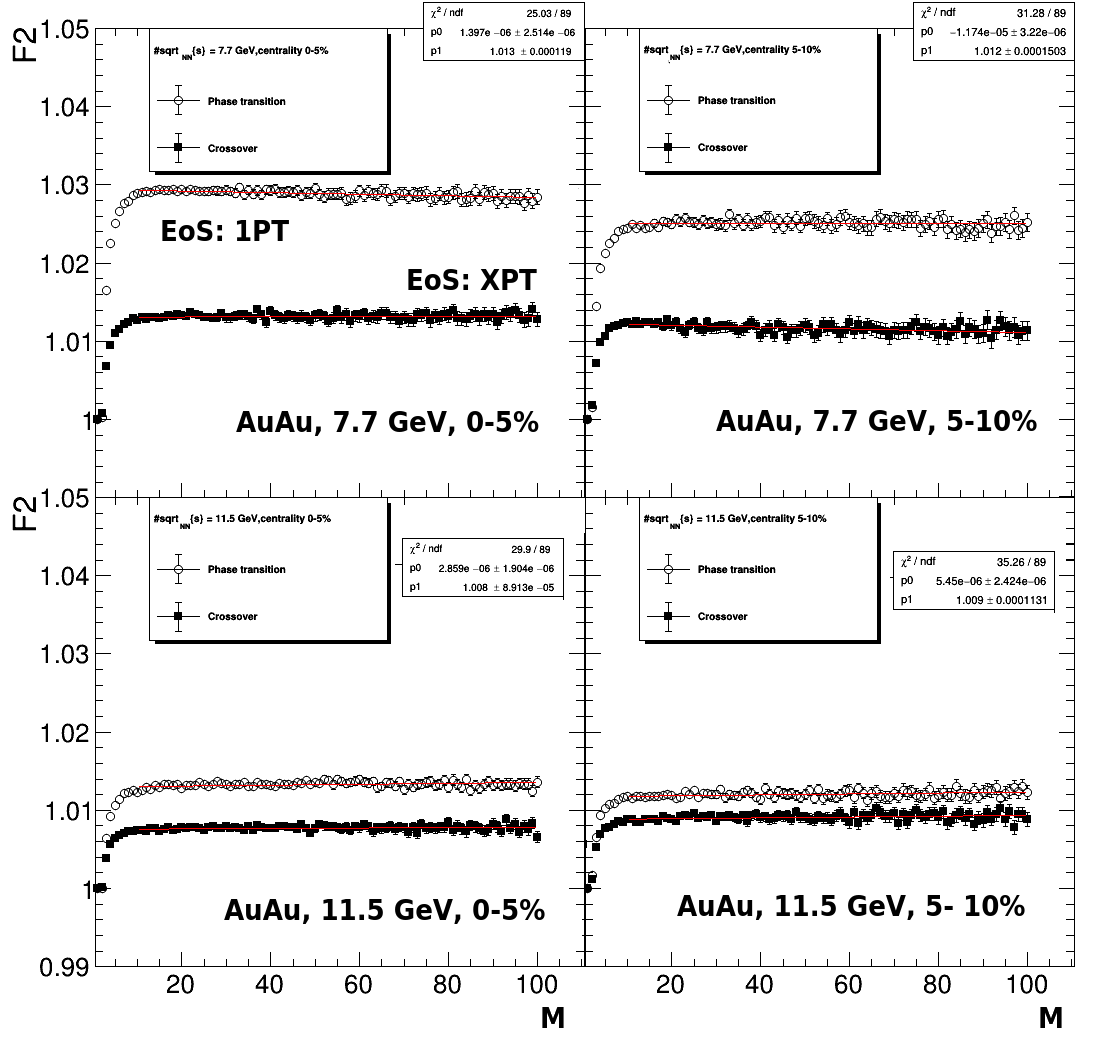
\includegraphics[width=1.\linewidth]{factorialMoments.png}             
            \end{figure}
            \column{.05\textwidth}
          \end{columns}
        \end{frame}

        \begin{frame}
          \frametitle{\bf \centering Factorial moments with vHLLE+UrQMD}
          \vskip -.5cm
          \begin{columns}[t]
             \column{.05\textwidth}
            \column{.7\textwidth}
            \begin{block}{}
              \begin{figure}[H]
                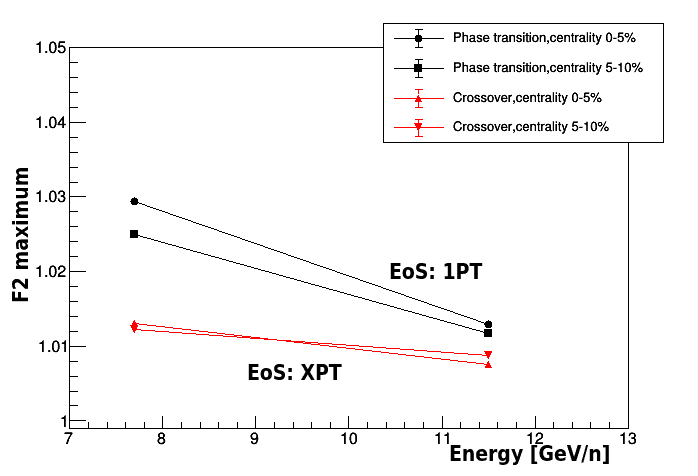
\includegraphics[width=1.\linewidth]{F2Max_enegyDep.png}             
              \end{figure}
            \end{block}
             \column{.05\textwidth}
          \end{columns}
          \begin{block}{}
            \bf \color {darkred!70!black} Different energy dependence is expected for XPT and 1PT EoS
            \end{block}
        \end{frame}

         \begin{frame}[shrink]
        \frametitle{\bf \centering Probing $\Delta \eta$-$\Delta \phi^{*}$ with MPD reconstructed tracks}
        \bf
        \vskip -0.3cm
        \begin{block}{}
          \vskip -.3cm
             \begin{equation*}
               \Delta \phi^{*} = \phi_{1} - \phi_{2} + \arcsin \left (\dfrac{z \cdot e \cdot B_{z} \cdot R}{2p_{T1}} \right) -
               \arcsin \left (\dfrac{z \cdot e \cdot B_{z} \cdot R}{2p_{T2}} \right)
             \end{equation*}
        \end{block}
        \begin{block}{}
          $R$ is a given cylindrical radius \\
          $\phi_{1, 2}$ are azimuthal angles of track at reconstructed vertex
          
        \end{block}
        \begin{block}{}
           \begin{figure}[H]
             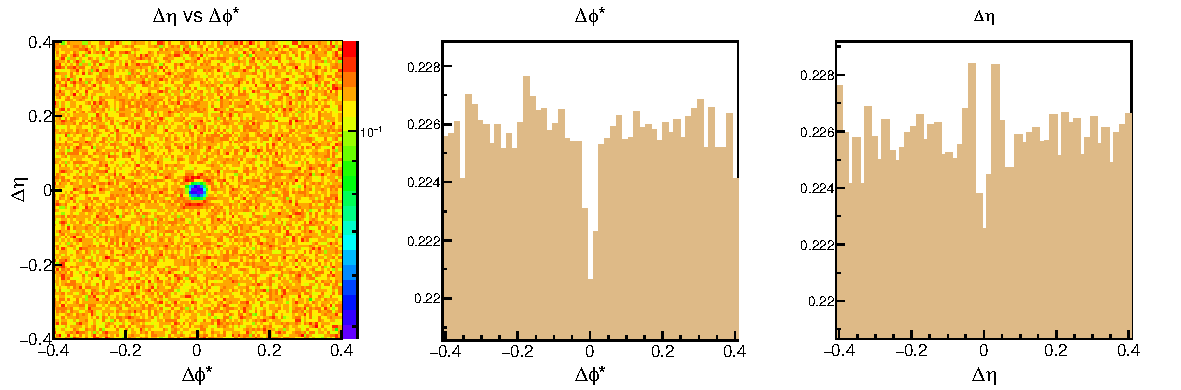
\includegraphics[width=1.\linewidth]{NICAdays_dEtadPhis.pdf}
           \end{figure}
        \end{block}
             
         \end{frame}

         \begin{frame}
           \frametitle{\bf \centering \footnotesize Probing $\Delta \eta$-$\Delta \phi^{*}$ with MPD reconstructed 1D-correlation function}
           %\begin{block}{}
              \begin{figure}[H]
            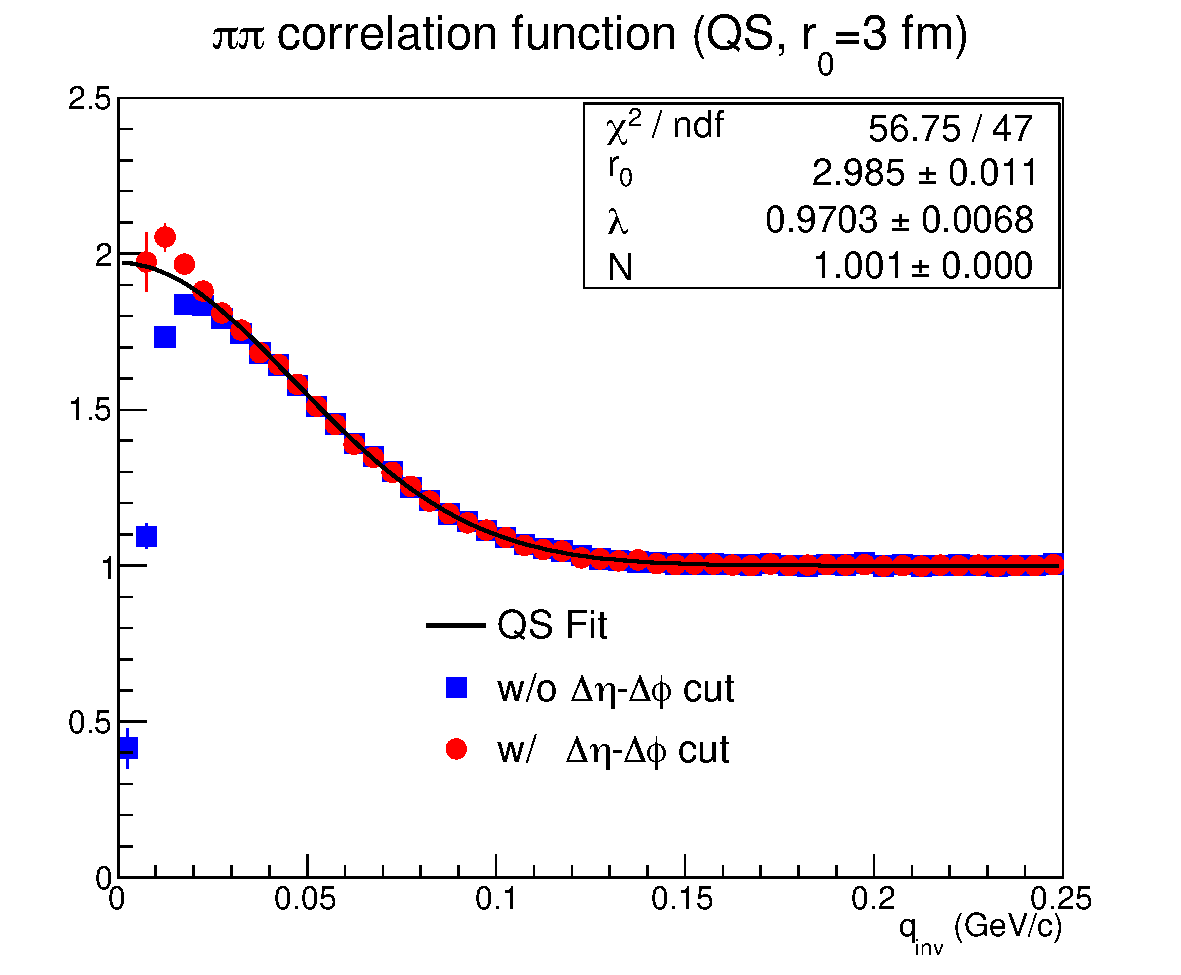
\includegraphics[width=.75\linewidth]{cfTest_new.pdf}
          \end{figure}
           %\end{block}
         \end{frame}
        
        \begin{frame}
          \frametitle{}
          \bf
          \begin{center}
            \Huge {Other activities we do}
          \end{center}
        \end{frame}

        \begin{frame}[fragile]
  \bf
  \frametitle{\bf \centering vHLLE+UrQMD interface software}
  \begin{block}{\bf \centering \color{darkred!70!black} How to get?}
    \scriptsize
       \begin{lstlisting}[language=C++,basicstyle=\ttfamily,keywordstyle=\color{darkred!70!black}]
         1. git clone https://github.com/pbatyuk/vHLLE_package.git
         2. git checkout 1.1.2
       \end{lstlisting}
  \end{block}
  \begin{block}{\bf \centering \color{darkred!70!black} How to compile and use?}
    \begin{itemize}
      \item vHLLE\_package/README.md (very detailed description on how to ...) 
    \end{itemize}
  \end{block}
   \begin{block}{\bf \centering \color{darkred!70!black} Aim of the project:}
     \begin{itemize}
     \item To collect all components (model + interface) in one place.
    \item To start simulations locally or remotely in a common way.
    \item To avoid a huge messy in the start configure scripts.
      \item {\color {darkblue!70!black} Possibility to use the model for its adjustment (pre-hydro + hydro phase)} as planned.
    \end{itemize}
  \end{block}
\end{frame}

\begin{frame}[fragile]
  \frametitle{\bf \centering \scriptsize vHLLE+UrQMD interface software}
  \vskip -.3cm
  \begin{block}{\bf \centering \color{darkred!70!black} \scriptsize Main macro: vHLLE\_package/macro/vHLLE.C}
    \vskip -.75cm
    \tiny
    \begin{lstlisting}[language=C++,basicstyle=\ttfamily,keywordstyle=\color{darkred!70!black}]

void vHLLE() {
VHLLE* gen = new VHLLE();
gen->SetSourceROOT(""); // Set ROOT-environment if not set yet and necessary to be set
// gen->SetExtendedFileName(kTRUE); // Set use of extended output filename ...
gen->SetUseBatch(kFALSE); // False value (default) means calculations at your locale machine ...
gen->SetBatchCluster("ncx"); // Possible values are: ncx, govorun, basov and gsi
    
// Parameters below (6) are considered as those to be set obligatory
gen->SetPathToTheModel(""); // Absolute(!) path to the root folder of the model
gen->SetOutputDirectory(""); // Directory where output data stored
gen->SetEnergy(7.7); // Set collision energy [GeV], possible energies are 7.7 GeV ...
gen->SetImpact(0., 3.3); // Set impact range (min, max) [fm]
gen->SetEoS("XPT"); // Set EoS to be used (1PT - first order phase transition, XPT - crossover)
gen->SetNsamples(100); // nEvents to be sampled in hadronic cascade from one hydro-evolution
    
gen->SetParameters(); // Set parameters for urqmd, hydro and hadronic cascade given by ...
    
// Modifiers to redefine almost all parameters given by the author for urqmd, hydro ...
// See $VHLLE/vhlle.h to get more if needed
// N. B.: Redefinition, if needed, can be done after gen->SetParameters() called !!! 
/*
gen->SetTau0(3.2);      
gen->SetEtaS(0.2);
gen->SetRg(1.4);
gen->SetRgz(0.5);
gen->SetNsamples(100);
*/

gen->PrintBasicParams();
gen->CheckParamsValidity(); // It checks whether the params defined are consistent
gen->GenerateStartScript(); // It produces a script to be executed
delete gen;
}
    \end{lstlisting}
  \end{block} 
\end{frame}

         \begin{frame}
        \bf
        \frametitle{\bf \centering Package for Femtoscopic Analysis}
        \vskip -0.8cm
        \begin{columns}[t]
          \column{.49\textwidth}
          \begin{block}{\bf \centering {\footnotesize {\color{darkred!70!black} Femtoscopy}}}
            \begin{itemize}
            \item \scriptsize Inherited from STAR (StHbtMaker) and ALICE (AliFemto)
            \item \scriptsize Keeps the same hierarchy as in ALICE (PckgName/, PckgNameUser/, macros/)
            \item \scriptsize Works with ROOT 5 and 6
            \item  \scriptsize Lighter than ancestors:
              \begin{itemize}
              \item \scriptsize Most of STAR-developed classes replaced with ROOT ones
              \item \scriptsize Better compression, smaller sizes
              \end{itemize}
            \item \scriptsize Implemented running options (INDEPENDENT on experiment-dependent software):
              \begin{itemize}
              \item \scriptsize Standalone mode – compile with g++ (clang) and run on your “laptop”
              \item \scriptsize Maker; Tasks will be also implemented
              \end{itemize}
            \end{itemize}
          \end{block}

          \column{.49\textwidth}
          \begin{block}{\bf \centering {\footnotesize {\color{darkgreen!50!black} Data formats (DST)}}}
            \begin{itemize}
            \item  \footnotesize General-purpose data format for Monte Carlo generators - McDst
            \item  \footnotesize Similar to UniGen (developed at GSI)
            \item  \footnotesize Lighter, faster, easy expandable, works with ROOT 5 and 6, g++ (clang)
            \item  \footnotesize Possibility to add converters from other generators: Terminator, EPOS, AMPT ...
            \item  \footnotesize Group has a positive experience on the data format developments:
              \begin{itemize}
              \item  \footnotesize PicoDst format in STAR (standard data format for physics analysis)
              \end{itemize}
            \end{itemize}
          \end{block}
          \vskip -.4cm
          \begin{block}{}
            \bf
            \color{darkred!70!black} \scriptsize Needed raw information from generator on momentum and coordinates! 
          \end{block}
        \end{columns}
      \end{frame}

      \begin{frame}[fragile]
        \bf
        \frametitle{\bf \centering Package for Femtoscopic Analysis}
        \vskip -.83cm
        \begin{columns}[t]
          \column{.58\textwidth}
          \begin{block}{\bf \centering \scriptsize Output ROOT tree:}
            \begin{figure}[H]
              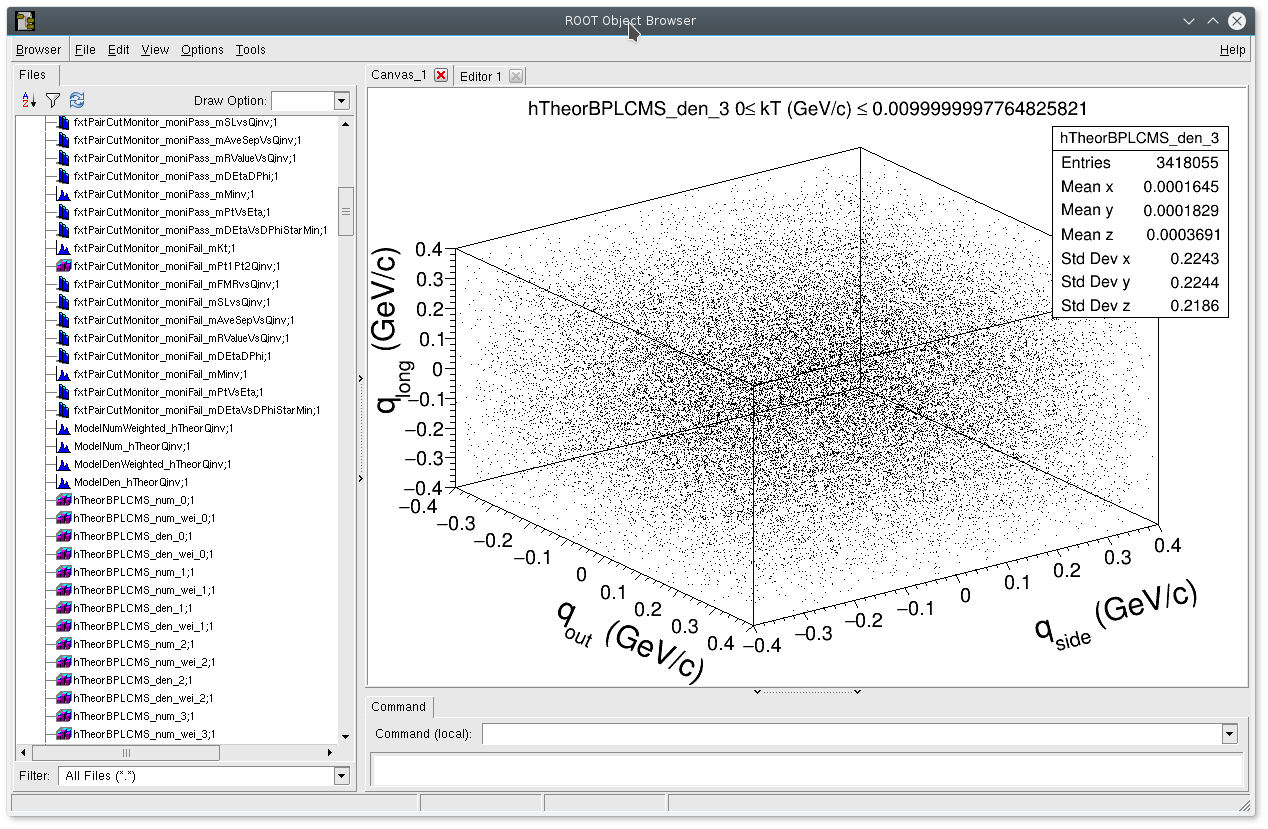
\includegraphics[width=1.\linewidth]{FemtoPack_example.png}
            \end{figure}
          \end{block}
          \vskip -0.3cm
          \begin{block}{\bf \centering \scriptsize It allows:}
            \begin{itemize}
            \item \scriptsize To set track cuts, particle pair cuts, number of events to be used for mixing ...
            \item \scriptsize To get 1D and 3D correlation functions for a set of $k_{T}$-bins
            \item \scriptsize To switch on / off different physics effects (QS, FSI ...)
            \end{itemize}
          \end{block}

          \column{.41\textwidth}
          \begin{block}{\bf \centering \tiny Main macro to define conditions of user's analysis}
            \vskip -0.33cm
                   {\tiny
                     \begin{lstlisting}[language=C++,basicstyle=\tiny\ttfamily,keywordstyle=\color{darkred!70!black}]
int main(int argc, char* argv[]) {
...
 // Create and set track cut
trackCut->setPdgId(particlePdg);
trackCut->setEta(-1., 1.);
trackCut->setPt(0.15, 1.55);
trackCut->setMass(particleMass);
...
// Set how many events to mix
hbtAnalysis->setNumEventsToMix(10);
...
// Lednicky weight generator
hbtWeight->setPairType(pairType);
hbtWeight->setCoulOn();
hbtWeight->setQuantumOn();
hbtWeight->setStrongOff();
hbtWeight->set3BodyOff();
...
// Create 1D correlation function
// integrated over kT
StHbtModelQinvCorrFctn *oneDim =
new StHbtModelQinvCorrFctn
("hTheorQinv", 40, 0., 0.4);
// Create 3D correlation function
// integrated with kT binning
StHbtModelBPLCMS3DCorrFctnKt *threeDim =
new StHbtModelBPLCMS3DCorrFctnKt
("hTheorBPLCMS", 80, -0.4, 0.4, 4,
0.15, 0.59);
}
\end{lstlisting}
}
\end{block}
\end{columns}     
      \end{frame}

\begin{frame}[fragile]
  \frametitle{\bf \centering MiniDST, current status}
\vskip -0.2cm
  %  \column{.49\textwidth}
    \begin{block}{\bf \centering \color{darkred!70!black} How to get?}
      \scriptsize
       \begin{lstlisting}[language=C++,basicstyle=\ttfamily,keywordstyle=\color{darkred!70!black}]
         1. git clone --recursive https://git.jinr.ru/nica/mpdroot.git
         2. git checkout miniDST_toBeTested
       \end{lstlisting}
    \end{block}

    \begin{block}{\bf \centering \color{darkred!70!black} Source codes in MpdRoot:}
      \bf \footnotesize
       \begin{itemize}
       \item {\color{darkblue!70!black} MiniDST source codes:} \$VMCWORKDIR/mpddst/MpdMiniEvent/MpdMini*.h(cxx) -
       \item {\color{darkblue!70!black} Converter to the format:} \$VMCWORKDIR/mpddst/MpdMiniDstFillTask.h(cxx)
       \end{itemize}
     \end{block}

    \begin{block}{\bf \centering \color{darkred!70!black} Use in reco.C:}
      \vskip -.75cm
      \scriptsize
        \begin{lstlisting}[language=C++,basicstyle=\ttfamily,keywordstyle=\color{darkred!70!black}]
...
// Task to be included
MpdMiniDstFillTask* miniDst = new MpdMiniDstFillTask("miniDST.root");
// miniDst->isUseTpc(kFALSE);
// miniDst->isUseTof(kFALSE);
// miniDst->isUseEcal(kTRUE);
miniDst->isUseMcTracks(kTRUE);
fRun->AddTask(miniDst);
...
        \end{lstlisting}
        
    \end{block} 
\end{frame}

\begin{frame}
  \bf
  \footnotesize
  \frametitle{\bf \centering MiniDST, current status}
  \begin{columns}
    \column{.49\textwidth}
    \begin{block}{\bf \centering \color{darkred!70!black} Already done:}
      \begin{itemize}
      \item Output data format derived from STAR has been incorporated to MpdRoot.
      \item Converter to be used for filling the format, written in a ``canonical way''
        via the FairRoot task mechanism, has been incorporated to MpdRoot.
      \item Some data members of the format have been already filled.
      \item The task has been added to the main reco macro.
      \item The task allows one to include / exclude detectors (data types - MC or reco) to be written to output.  
      \end{itemize}     
    \end{block}
  
    \column{.49\textwidth}
    \begin{block}{\bf \centering \color{darkblue!70!black} Planned to be done a.s.a.p.:}
      \begin{itemize}
      \item To fill remaining data members of the format (A discussion required ...).
      \item To decide whether we need to add new or remove existing data members or not to be adopted better to MPD.
      \item To extend the format by specific detectors to be used in MPD.
      \item ...
      \item {\color{darkred!70!black} As done and extensively tested, to finish transition to the format as the main output from reco.}
        (Right now a standard DST and the current one co-exist together)
      \end{itemize} 
    \end{block}    
  \end{columns} 
\end{frame}
      
      \begin{frame}
        \frametitle{}
        \begin{center}
          \bf
          \Huge {Thank you for attention!}
        \end{center}
      \end{frame}
      
      \end{document}
      
